\hypertarget{_lgm___c_trans_8c}{
\section{/home/mgh/LanlGeoMag/libLanlGeoMag/Lgm\_\-CTrans.c File Reference}
\label{_lgm___c_trans_8c}\index{/home/mgh/LanlGeoMag/libLanlGeoMag/Lgm\_\-CTrans.c@{/home/mgh/LanlGeoMag/libLanlGeoMag/Lgm\_\-CTrans.c}}
}
{\tt \#include \char`\"{}Lgm/Lgm\_\-CTrans.h\char`\"{}}\par
{\tt \#include \char`\"{}Lgm/Lgm\_\-Quat.h\char`\"{}}\par
{\tt \#include $<$ctype.h$>$}\par
{\tt \#include $<$time.h$>$}\par


Include dependency graph for Lgm\_\-CTrans.c:\nopagebreak
\begin{figure}[H]
\begin{center}
\leavevmode
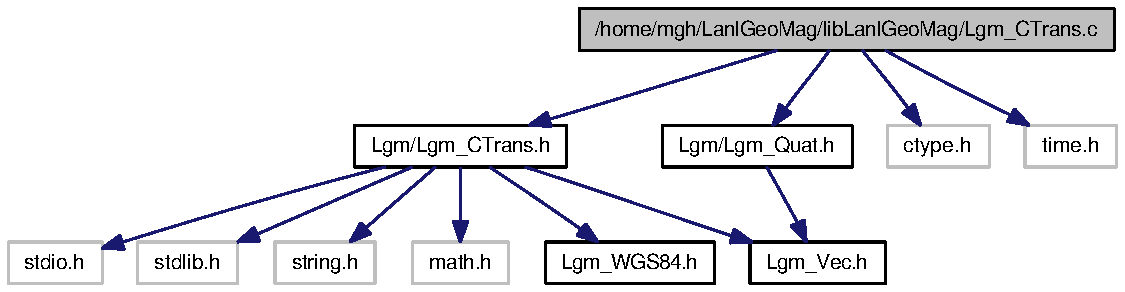
\includegraphics[width=288pt]{_lgm___c_trans_8c__incl}
\end{center}
\end{figure}
\subsection*{Defines}
\begin{CompactItemize}
\item 
\#define \hyperlink{_lgm___c_trans_8c_39e10ff200010833ffe9d6471a777192}{USE\_\-HIGH\_\-ACCURACY\_\-SUN}~1
\item 
\#define \hyperlink{_lgm___c_trans_8c_d8a5aea0c56b658d9939ad14b376ca9d}{LGM\_\-EOP\_\-DATA\_\-DIR}~/usr/local/share/LanlGeoMag/EopData
\end{CompactItemize}
\subsection*{Functions}
\begin{CompactItemize}
\item 
void \hyperlink{_lgm___c_trans_8c_5434c56ab7ae78cd7186d0c9dc17004c}{Lgm\_\-free\_\-ctrans} (\hyperlink{struct_lgm___c_trans}{Lgm\_\-CTrans} $\ast$c)
\item 
\hyperlink{struct_lgm___c_trans}{Lgm\_\-CTrans} $\ast$ \hyperlink{_lgm___c_trans_8c_73c768f9cf06f4f95be0aa829c10d02c}{Lgm\_\-init\_\-ctrans} (int Verbose)
\item 
\hyperlink{struct_lgm___c_trans}{Lgm\_\-CTrans} $\ast$ \hyperlink{_lgm___c_trans_8c_7278ce0ecd85d19b95770c9ef37b07c3}{Lgm\_\-CopyCTrans} (\hyperlink{struct_lgm___c_trans}{Lgm\_\-CTrans} $\ast$s)
\begin{CompactList}\small\item\em The \hyperlink{struct_lgm___c_trans}{Lgm\_\-CTrans} structure has pointers in it, so simple asignments (e.g. \item\end{CompactList}\item 
void \hyperlink{_lgm___c_trans_8c_c3269f332d380c33fb005f1911cad403}{Lgm\_\-Radec\_\-to\_\-Cart} (double ra, double dec, \hyperlink{struct_lgm___vector}{Lgm\_\-Vector} $\ast$r)
\begin{CompactList}\small\item\em Converts RA and DEC to unit vector in cartesian coords. \item\end{CompactList}\item 
double \hyperlink{_lgm___c_trans_8c_d537aa2aa2d71d12230e47b051a40a69}{Lgm\_\-angle2pi} (double angle)
\item 
double \hyperlink{_lgm___c_trans_8c_b87401a0610af3447b91b2eee720d8ac}{Lgm\_\-angle360} (double angle)
\item 
long int \hyperlink{_lgm___c_trans_8c_4a4b0532bf6fb44bc8d4d9fbbab0d5cf}{Lgm\_\-JD\_\-to\_\-Date} (double jd, int $\ast$ny, int $\ast$nm, int $\ast$nd, double $\ast$UT)
\begin{CompactList}\small\item\em Compute the Julian Day number for the given date. \item\end{CompactList}\item 
long int \hyperlink{_lgm___c_trans_8c_49849aa31ba274bbc716a453f4629724}{Lgm\_\-MJD\_\-to\_\-Date} (double mjd, int $\ast$ny, int $\ast$nm, int $\ast$nd, double $\ast$UT)
\item 
double \hyperlink{_lgm___c_trans_8c_5c4772e1bd79501232af313899c1814a}{Lgm\_\-hour24} (double hour)
\item 
double \hyperlink{_lgm___c_trans_8c_59884535937bd9e67beca41c68aa0864}{Lgm\_\-kepler} (double M, double e)
\item 
void \hyperlink{_lgm___c_trans_8c_60cb99abfbae34ae5e7a41c797dcac0e}{Lgm\_\-Set\_\-Coord\_\-Transforms} (long int date, double UTC, \hyperlink{struct_lgm___c_trans}{Lgm\_\-CTrans} $\ast$c)
\item 
void \hyperlink{_lgm___c_trans_8c_3975f7cfbe7332bf9b471532d496f442}{Lgm\_\-Convert\_\-Coords} (\hyperlink{struct_lgm___vector}{Lgm\_\-Vector} $\ast$u, \hyperlink{struct_lgm___vector}{Lgm\_\-Vector} $\ast$v, int flag, \hyperlink{struct_lgm___c_trans}{Lgm\_\-CTrans} $\ast$c)
\item 
void \hyperlink{_lgm___c_trans_8c_765b74946e14a91f17fdb32761073682}{Lgm\_\-GEOD\_\-to\_\-WGS84} (double GeodLat, double GeodLong, double GeodHeight, \hyperlink{struct_lgm___vector}{Lgm\_\-Vector} $\ast$v)
\item 
void \hyperlink{_lgm___c_trans_8c_64e411cdf591772fca631d5e42fdacd3}{Lgm\_\-WGS84\_\-to\_\-GEOD} (\hyperlink{struct_lgm___vector}{Lgm\_\-Vector} $\ast$uin, double $\ast$GeodLat, double $\ast$GeodLong, double $\ast$GeodHeight)
\item 
void \hyperlink{_lgm___c_trans_8c_323f92aef0fee19b69f4da4684fb821c}{Lgm\_\-WGS84\_\-to\_\-GeodHeight} (\hyperlink{struct_lgm___vector}{Lgm\_\-Vector} $\ast$uin, double $\ast$GeodHeight)
\item 
void \hyperlink{_lgm___c_trans_8c_4e7b063e0734746ff6af5ef5118ed8b8}{Lgm\_\-B\_\-igrf\_\-ctrans} (\hyperlink{struct_lgm___vector}{Lgm\_\-Vector} $\ast$v, \hyperlink{struct_lgm___vector}{Lgm\_\-Vector} $\ast$B, \hyperlink{struct_lgm___c_trans}{Lgm\_\-CTrans} $\ast$c)
\item 
void \hyperlink{_lgm___c_trans_8c_a23fbb09653a52bfb6e38be64231ad8d}{Lgm\_\-B\_\-cdip\_\-ctrans} (\hyperlink{struct_lgm___vector}{Lgm\_\-Vector} $\ast$v, \hyperlink{struct_lgm___vector}{Lgm\_\-Vector} $\ast$B, \hyperlink{struct_lgm___c_trans}{Lgm\_\-CTrans} $\ast$c)
\item 
void \hyperlink{_lgm___c_trans_8c_5302ef2d070d2764b911aac4cbd2f4f0}{Lgm\_\-B\_\-edip\_\-ctrans} (\hyperlink{struct_lgm___vector}{Lgm\_\-Vector} $\ast$v, \hyperlink{struct_lgm___vector}{Lgm\_\-Vector} $\ast$B, \hyperlink{struct_lgm___c_trans}{Lgm\_\-CTrans} $\ast$c)
\item 
void \hyperlink{_lgm___c_trans_8c_8235053e9b85c2b8573f4631df5406a1}{Lgm\_\-jd\_\-to\_\-ymdh} (double JD, long int $\ast$Date, int $\ast$year, int $\ast$month, int $\ast$day, double $\ast$UT)
\item 
void \hyperlink{_lgm___c_trans_8c_18027f421b92398b5b8c53915f340759}{Lgm\_\-mjd\_\-to\_\-ymdh} (double MJD, long int $\ast$Date, int $\ast$year, int $\ast$month, int $\ast$day, double $\ast$UT)
\item 
void \hyperlink{_lgm___c_trans_8c_66b28744847e26256778562fd41d07fb}{Lgm\_\-UT\_\-to\_\-hmsms} (double UT, int $\ast$Hour, int $\ast$Min, int $\ast$Sec, int $\ast$MilliSec)
\item 
void \hyperlink{_lgm___c_trans_8c_4c5eb958c42764eb7c98c2209a191d6e}{Lgm\_\-UT\_\-to\_\-HMS} (double UT, int $\ast$HH, int $\ast$MM, int $\ast$SS)
\item 
void \hyperlink{_lgm___c_trans_8c_df736dd325580fae9f0bd5fde0fab40e}{Lgm\_\-UT\_\-to\_\-HMSd} (double UT, int $\ast$sgn, int $\ast$HH, int $\ast$MM, double $\ast$SS)
\item 
void \hyperlink{_lgm___c_trans_8c_44f52ee0cf2a11d21329cc7d65448840}{Lgm\_\-D\_\-to\_\-DMS} (double D, int $\ast$DD, int $\ast$MM, int $\ast$SS)
\item 
void \hyperlink{_lgm___c_trans_8c_0366f317f96ffed4e998ce1551d5c190}{Lgm\_\-D\_\-to\_\-DMSd} (double D, int $\ast$sgn, int $\ast$DD, int $\ast$MM, double $\ast$SS)
\item 
double \hyperlink{_lgm___c_trans_8c_8282c3981409facddb1146c8a38a6473}{Lgm\_\-GetCurrentJD} (\hyperlink{struct_lgm___c_trans}{Lgm\_\-CTrans} $\ast$c)
\item 
double \hyperlink{_lgm___c_trans_8c_cb69b434aa7af16c67eadb8679d700fc}{Lgm\_\-GetCurrentMJD} (\hyperlink{struct_lgm___c_trans}{Lgm\_\-CTrans} $\ast$c)
\item 
void \hyperlink{_lgm___c_trans_8c_020fa6e5734e315d2fc9d982263a0f32}{Lgm\_\-Print\_\-HMS} (double d)
\item 
void \hyperlink{_lgm___c_trans_8c_8c54f2ea495708f306d69eb5cbd5407f}{Lgm\_\-Print\_\-HMSdp} (double d, int UnicodeHMS, int p)
\item 
void \hyperlink{_lgm___c_trans_8c_09be79dfd1f30dc8313931e19bfb2b68}{Lgm\_\-Print\_\-HMSd} (double d)
\item 
void \hyperlink{_lgm___c_trans_8c_c0752451ba731db6f7ad5ff7aa7388cb}{Lgm\_\-Print\_\-DMS} (double d)
\item 
void \hyperlink{_lgm___c_trans_8c_0f6fd0c4c8d56743de4c9e24039eb1df}{Lgm\_\-Print\_\-DMSd} (double d)
\item 
void \hyperlink{_lgm___c_trans_8c_022c69d1faa38210aba90d732e3b4327}{Lgm\_\-CDMAG\_\-to\_\-R\_\-MLAT\_\-MLON\_\-MLT} (\hyperlink{struct_lgm___vector}{Lgm\_\-Vector} $\ast$u, double $\ast$R, double $\ast$MLAT, double $\ast$MLON, double $\ast$MLT, \hyperlink{struct_lgm___c_trans}{Lgm\_\-CTrans} $\ast$c)
\item 
void \hyperlink{_lgm___c_trans_8c_b266f1ac29eac32ae2bc43c92514a8c1}{Lgm\_\-R\_\-MLAT\_\-MLT\_\-to\_\-CDMAG} (double R, double MLAT, double MLT, \hyperlink{struct_lgm___vector}{Lgm\_\-Vector} $\ast$u, \hyperlink{struct_lgm___c_trans}{Lgm\_\-CTrans} $\ast$c)
\item 
void \hyperlink{_lgm___c_trans_8c_ffd68c7f63f3835e4b941894d7970036}{Lgm\_\-EDMAG\_\-to\_\-R\_\-MLAT\_\-MLON\_\-MLT} (\hyperlink{struct_lgm___vector}{Lgm\_\-Vector} $\ast$u, double $\ast$R, double $\ast$MLAT, double $\ast$MLON, double $\ast$MLT, \hyperlink{struct_lgm___c_trans}{Lgm\_\-CTrans} $\ast$c)
\item 
void \hyperlink{_lgm___c_trans_8c_990e8076d81fa9fb61683eadba58f948}{Lgm\_\-R\_\-MLAT\_\-MLT\_\-to\_\-EDMAG} (double R, double MLAT, double MLT, \hyperlink{struct_lgm___vector}{Lgm\_\-Vector} $\ast$u, \hyperlink{struct_lgm___c_trans}{Lgm\_\-CTrans} $\ast$c)
\item 
void \hyperlink{_lgm___c_trans_8c_ac416039271e229bfe94fd9f7b610dc5}{Lgm\_\-GLATLON\_\-TO\_\-CDMLATLONMLT} (double GLAT, double GLON, double $\ast$MLAT, double $\ast$MLON, double $\ast$MLT, \hyperlink{struct_lgm___c_trans}{Lgm\_\-CTrans} $\ast$c)
\item 
void \hyperlink{_lgm___c_trans_8c_cd9faa6a7bfbe63a8b4ece64e9940d3d}{Lgm\_\-GLATLON\_\-TO\_\-EDMLATLONMLT} (double GLAT, double GLON, double $\ast$MLAT, double $\ast$MLON, double $\ast$MLT, \hyperlink{struct_lgm___c_trans}{Lgm\_\-CTrans} $\ast$c)
\item 
void \hyperlink{_lgm___c_trans_8c_6451734bb5156adb8f3dcff4f699f6c6}{ParseTimeStr} (char $\ast$Str, int $\ast$Year, int $\ast$Month, int $\ast$Day, int $\ast$hh, int $\ast$mm, double $\ast$ss, long int $\ast$Date, double $\ast$H)
\item 
int \hyperlink{_lgm___c_trans_8c_d1aa3133c642d6449d82195218a982d7}{MonthStrToNum} (char $\ast$str)
\item 
char $\ast$ \hyperlink{_lgm___c_trans_8c_a235edbf150af5c6ad528c6a6f549776}{Lgm\_\-StrToLower} (char $\ast$str, int nmax)
\item 
char $\ast$ \hyperlink{_lgm___c_trans_8c_aab1a57905dff35bc1efeef8c3f6a576}{Lgm\_\-StrToUpper} (char $\ast$str, int nmax)
\end{CompactItemize}


\subsection{Define Documentation}
\hypertarget{_lgm___c_trans_8c_39e10ff200010833ffe9d6471a777192}{
\index{Lgm\_\-CTrans.c@{Lgm\_\-CTrans.c}!USE\_\-HIGH\_\-ACCURACY\_\-SUN@{USE\_\-HIGH\_\-ACCURACY\_\-SUN}}
\index{USE\_\-HIGH\_\-ACCURACY\_\-SUN@{USE\_\-HIGH\_\-ACCURACY\_\-SUN}!Lgm_CTrans.c@{Lgm\_\-CTrans.c}}
\subsubsection[{USE\_\-HIGH\_\-ACCURACY\_\-SUN}]{\setlength{\rightskip}{0pt plus 5cm}\#define USE\_\-HIGH\_\-ACCURACY\_\-SUN~1}}
\label{_lgm___c_trans_8c_39e10ff200010833ffe9d6471a777192}




Definition at line 6 of file Lgm\_\-CTrans.c.\hypertarget{_lgm___c_trans_8c_d8a5aea0c56b658d9939ad14b376ca9d}{
\index{Lgm\_\-CTrans.c@{Lgm\_\-CTrans.c}!LGM\_\-EOP\_\-DATA\_\-DIR@{LGM\_\-EOP\_\-DATA\_\-DIR}}
\index{LGM\_\-EOP\_\-DATA\_\-DIR@{LGM\_\-EOP\_\-DATA\_\-DIR}!Lgm_CTrans.c@{Lgm\_\-CTrans.c}}
\subsubsection[{LGM\_\-EOP\_\-DATA\_\-DIR}]{\setlength{\rightskip}{0pt plus 5cm}\#define LGM\_\-EOP\_\-DATA\_\-DIR~/usr/local/share/LanlGeoMag/EopData}}
\label{_lgm___c_trans_8c_d8a5aea0c56b658d9939ad14b376ca9d}




Definition at line 9 of file Lgm\_\-CTrans.c.

\subsection{Function Documentation}
\hypertarget{_lgm___c_trans_8c_5434c56ab7ae78cd7186d0c9dc17004c}{
\index{Lgm\_\-CTrans.c@{Lgm\_\-CTrans.c}!Lgm\_\-free\_\-ctrans@{Lgm\_\-free\_\-ctrans}}
\index{Lgm\_\-free\_\-ctrans@{Lgm\_\-free\_\-ctrans}!Lgm_CTrans.c@{Lgm\_\-CTrans.c}}
\subsubsection[{Lgm\_\-free\_\-ctrans}]{\setlength{\rightskip}{0pt plus 5cm}void Lgm\_\-free\_\-ctrans ({\bf Lgm\_\-CTrans} $\ast$ {\em c})}}
\label{_lgm___c_trans_8c_5434c56ab7ae78cd7186d0c9dc17004c}




Definition at line 14 of file Lgm\_\-CTrans.c.

Here is the caller graph for this function:\nopagebreak
\begin{figure}[H]
\begin{center}
\leavevmode
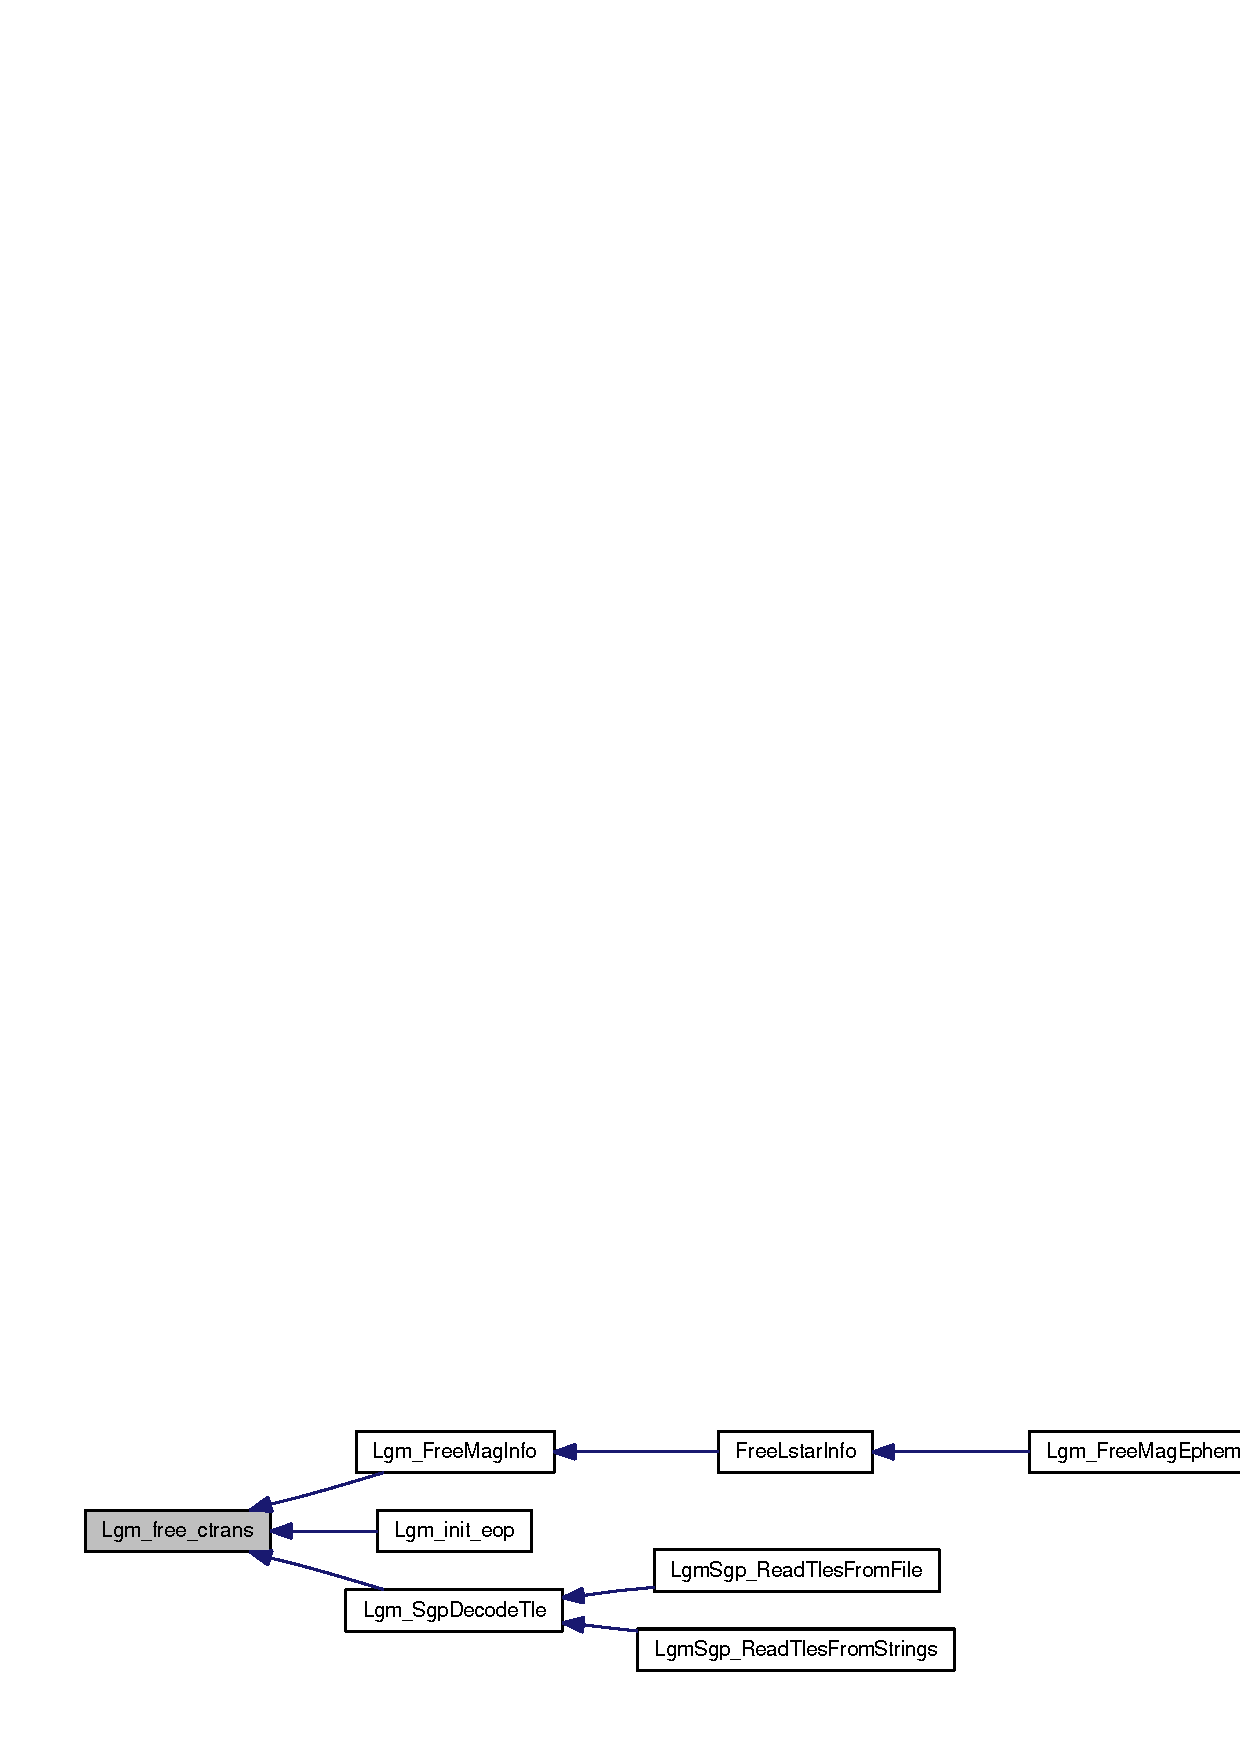
\includegraphics[width=312pt]{_lgm___c_trans_8c_5434c56ab7ae78cd7186d0c9dc17004c_icgraph}
\end{center}
\end{figure}
\hypertarget{_lgm___c_trans_8c_73c768f9cf06f4f95be0aa829c10d02c}{
\index{Lgm\_\-CTrans.c@{Lgm\_\-CTrans.c}!Lgm\_\-init\_\-ctrans@{Lgm\_\-init\_\-ctrans}}
\index{Lgm\_\-init\_\-ctrans@{Lgm\_\-init\_\-ctrans}!Lgm_CTrans.c@{Lgm\_\-CTrans.c}}
\subsubsection[{Lgm\_\-init\_\-ctrans}]{\setlength{\rightskip}{0pt plus 5cm}{\bf Lgm\_\-CTrans}$\ast$ Lgm\_\-init\_\-ctrans (int {\em Verbose})}}
\label{_lgm___c_trans_8c_73c768f9cf06f4f95be0aa829c10d02c}




Definition at line 27 of file Lgm\_\-CTrans.c.

Here is the call graph for this function:\nopagebreak
\begin{figure}[H]
\begin{center}
\leavevmode
\includegraphics[width=207pt]{_lgm___c_trans_8c_73c768f9cf06f4f95be0aa829c10d02c_cgraph}
\end{center}
\end{figure}


Here is the caller graph for this function:\nopagebreak
\begin{figure}[H]
\begin{center}
\leavevmode
\includegraphics[width=313pt]{_lgm___c_trans_8c_73c768f9cf06f4f95be0aa829c10d02c_icgraph}
\end{center}
\end{figure}
\hypertarget{_lgm___c_trans_8c_7278ce0ecd85d19b95770c9ef37b07c3}{
\index{Lgm\_\-CTrans.c@{Lgm\_\-CTrans.c}!Lgm\_\-CopyCTrans@{Lgm\_\-CopyCTrans}}
\index{Lgm\_\-CopyCTrans@{Lgm\_\-CopyCTrans}!Lgm_CTrans.c@{Lgm\_\-CTrans.c}}
\subsubsection[{Lgm\_\-CopyCTrans}]{\setlength{\rightskip}{0pt plus 5cm}{\bf Lgm\_\-CTrans}$\ast$ Lgm\_\-CopyCTrans ({\bf Lgm\_\-CTrans} $\ast$ {\em s})}}
\label{_lgm___c_trans_8c_7278ce0ecd85d19b95770c9ef37b07c3}


The \hyperlink{struct_lgm___c_trans}{Lgm\_\-CTrans} structure has pointers in it, so simple asignments (e.g. 

$\ast$t = $\ast$s) are dangerous. Here we make sure that the target gets an independent copy of the structure. 

Definition at line 68 of file Lgm\_\-CTrans.c.

Here is the caller graph for this function:\nopagebreak
\begin{figure}[H]
\begin{center}
\leavevmode
\includegraphics[width=205pt]{_lgm___c_trans_8c_7278ce0ecd85d19b95770c9ef37b07c3_icgraph}
\end{center}
\end{figure}
\hypertarget{_lgm___c_trans_8c_c3269f332d380c33fb005f1911cad403}{
\index{Lgm\_\-CTrans.c@{Lgm\_\-CTrans.c}!Lgm\_\-Radec\_\-to\_\-Cart@{Lgm\_\-Radec\_\-to\_\-Cart}}
\index{Lgm\_\-Radec\_\-to\_\-Cart@{Lgm\_\-Radec\_\-to\_\-Cart}!Lgm_CTrans.c@{Lgm\_\-CTrans.c}}
\subsubsection[{Lgm\_\-Radec\_\-to\_\-Cart}]{\setlength{\rightskip}{0pt plus 5cm}void Lgm\_\-Radec\_\-to\_\-Cart (double {\em ra}, \/  double {\em dec}, \/  {\bf Lgm\_\-Vector} $\ast$ {\em r})}}
\label{_lgm___c_trans_8c_c3269f332d380c33fb005f1911cad403}


Converts RA and DEC to unit vector in cartesian coords. 



Definition at line 114 of file Lgm\_\-CTrans.c.

Here is the caller graph for this function:\nopagebreak
\begin{figure}[H]
\begin{center}
\leavevmode
\includegraphics[width=267pt]{_lgm___c_trans_8c_c3269f332d380c33fb005f1911cad403_icgraph}
\end{center}
\end{figure}
\hypertarget{_lgm___c_trans_8c_d537aa2aa2d71d12230e47b051a40a69}{
\index{Lgm\_\-CTrans.c@{Lgm\_\-CTrans.c}!Lgm\_\-angle2pi@{Lgm\_\-angle2pi}}
\index{Lgm\_\-angle2pi@{Lgm\_\-angle2pi}!Lgm_CTrans.c@{Lgm\_\-CTrans.c}}
\subsubsection[{Lgm\_\-angle2pi}]{\setlength{\rightskip}{0pt plus 5cm}double Lgm\_\-angle2pi (double {\em angle})}}
\label{_lgm___c_trans_8c_d537aa2aa2d71d12230e47b051a40a69}




Definition at line 136 of file Lgm\_\-CTrans.c.

Here is the caller graph for this function:\nopagebreak
\begin{figure}[H]
\begin{center}
\leavevmode
\includegraphics[width=253pt]{_lgm___c_trans_8c_d537aa2aa2d71d12230e47b051a40a69_icgraph}
\end{center}
\end{figure}
\hypertarget{_lgm___c_trans_8c_b87401a0610af3447b91b2eee720d8ac}{
\index{Lgm\_\-CTrans.c@{Lgm\_\-CTrans.c}!Lgm\_\-angle360@{Lgm\_\-angle360}}
\index{Lgm\_\-angle360@{Lgm\_\-angle360}!Lgm_CTrans.c@{Lgm\_\-CTrans.c}}
\subsubsection[{Lgm\_\-angle360}]{\setlength{\rightskip}{0pt plus 5cm}double Lgm\_\-angle360 (double {\em angle})}}
\label{_lgm___c_trans_8c_b87401a0610af3447b91b2eee720d8ac}




Definition at line 153 of file Lgm\_\-CTrans.c.

Here is the caller graph for this function:\nopagebreak
\begin{figure}[H]
\begin{center}
\leavevmode
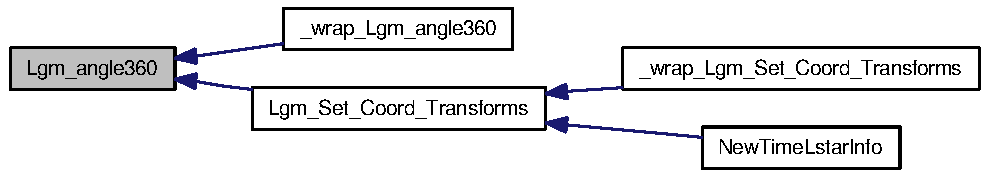
\includegraphics[width=255pt]{_lgm___c_trans_8c_b87401a0610af3447b91b2eee720d8ac_icgraph}
\end{center}
\end{figure}
\hypertarget{_lgm___c_trans_8c_4a4b0532bf6fb44bc8d4d9fbbab0d5cf}{
\index{Lgm\_\-CTrans.c@{Lgm\_\-CTrans.c}!Lgm\_\-JD\_\-to\_\-Date@{Lgm\_\-JD\_\-to\_\-Date}}
\index{Lgm\_\-JD\_\-to\_\-Date@{Lgm\_\-JD\_\-to\_\-Date}!Lgm_CTrans.c@{Lgm\_\-CTrans.c}}
\subsubsection[{Lgm\_\-JD\_\-to\_\-Date}]{\setlength{\rightskip}{0pt plus 5cm}long int Lgm\_\-JD\_\-to\_\-Date (double {\em jd}, \/  int $\ast$ {\em ny}, \/  int $\ast$ {\em nm}, \/  int $\ast$ {\em nd}, \/  double $\ast$ {\em UT})}}
\label{_lgm___c_trans_8c_4a4b0532bf6fb44bc8d4d9fbbab0d5cf}


Compute the Julian Day number for the given date. 

Julian Date is the number of days since noon of Jan 1 4713 B.C. 

Definition at line 175 of file Lgm\_\-CTrans.c.

Here is the caller graph for this function:\nopagebreak
\begin{figure}[H]
\begin{center}
\leavevmode
\includegraphics[width=420pt]{_lgm___c_trans_8c_4a4b0532bf6fb44bc8d4d9fbbab0d5cf_icgraph}
\end{center}
\end{figure}
\hypertarget{_lgm___c_trans_8c_49849aa31ba274bbc716a453f4629724}{
\index{Lgm\_\-CTrans.c@{Lgm\_\-CTrans.c}!Lgm\_\-MJD\_\-to\_\-Date@{Lgm\_\-MJD\_\-to\_\-Date}}
\index{Lgm\_\-MJD\_\-to\_\-Date@{Lgm\_\-MJD\_\-to\_\-Date}!Lgm_CTrans.c@{Lgm\_\-CTrans.c}}
\subsubsection[{Lgm\_\-MJD\_\-to\_\-Date}]{\setlength{\rightskip}{0pt plus 5cm}long int Lgm\_\-MJD\_\-to\_\-Date (double {\em mjd}, \/  int $\ast$ {\em ny}, \/  int $\ast$ {\em nm}, \/  int $\ast$ {\em nd}, \/  double $\ast$ {\em UT})}}
\label{_lgm___c_trans_8c_49849aa31ba274bbc716a453f4629724}




Definition at line 223 of file Lgm\_\-CTrans.c.

Here is the call graph for this function:\nopagebreak
\begin{figure}[H]
\begin{center}
\leavevmode
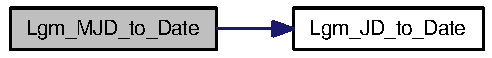
\includegraphics[width=136pt]{_lgm___c_trans_8c_49849aa31ba274bbc716a453f4629724_cgraph}
\end{center}
\end{figure}


Here is the caller graph for this function:\nopagebreak
\begin{figure}[H]
\begin{center}
\leavevmode
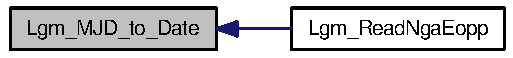
\includegraphics[width=141pt]{_lgm___c_trans_8c_49849aa31ba274bbc716a453f4629724_icgraph}
\end{center}
\end{figure}
\hypertarget{_lgm___c_trans_8c_5c4772e1bd79501232af313899c1814a}{
\index{Lgm\_\-CTrans.c@{Lgm\_\-CTrans.c}!Lgm\_\-hour24@{Lgm\_\-hour24}}
\index{Lgm\_\-hour24@{Lgm\_\-hour24}!Lgm_CTrans.c@{Lgm\_\-CTrans.c}}
\subsubsection[{Lgm\_\-hour24}]{\setlength{\rightskip}{0pt plus 5cm}double Lgm\_\-hour24 (double {\em hour})}}
\label{_lgm___c_trans_8c_5c4772e1bd79501232af313899c1814a}




Definition at line 227 of file Lgm\_\-CTrans.c.

Here is the caller graph for this function:\nopagebreak
\begin{figure}[H]
\begin{center}
\leavevmode
\includegraphics[width=420pt]{_lgm___c_trans_8c_5c4772e1bd79501232af313899c1814a_icgraph}
\end{center}
\end{figure}
\hypertarget{_lgm___c_trans_8c_59884535937bd9e67beca41c68aa0864}{
\index{Lgm\_\-CTrans.c@{Lgm\_\-CTrans.c}!Lgm\_\-kepler@{Lgm\_\-kepler}}
\index{Lgm\_\-kepler@{Lgm\_\-kepler}!Lgm_CTrans.c@{Lgm\_\-CTrans.c}}
\subsubsection[{Lgm\_\-kepler}]{\setlength{\rightskip}{0pt plus 5cm}double Lgm\_\-kepler (double {\em M}, \/  double {\em e})}}
\label{_lgm___c_trans_8c_59884535937bd9e67beca41c68aa0864}




Definition at line 241 of file Lgm\_\-CTrans.c.

Here is the caller graph for this function:\nopagebreak
\begin{figure}[H]
\begin{center}
\leavevmode
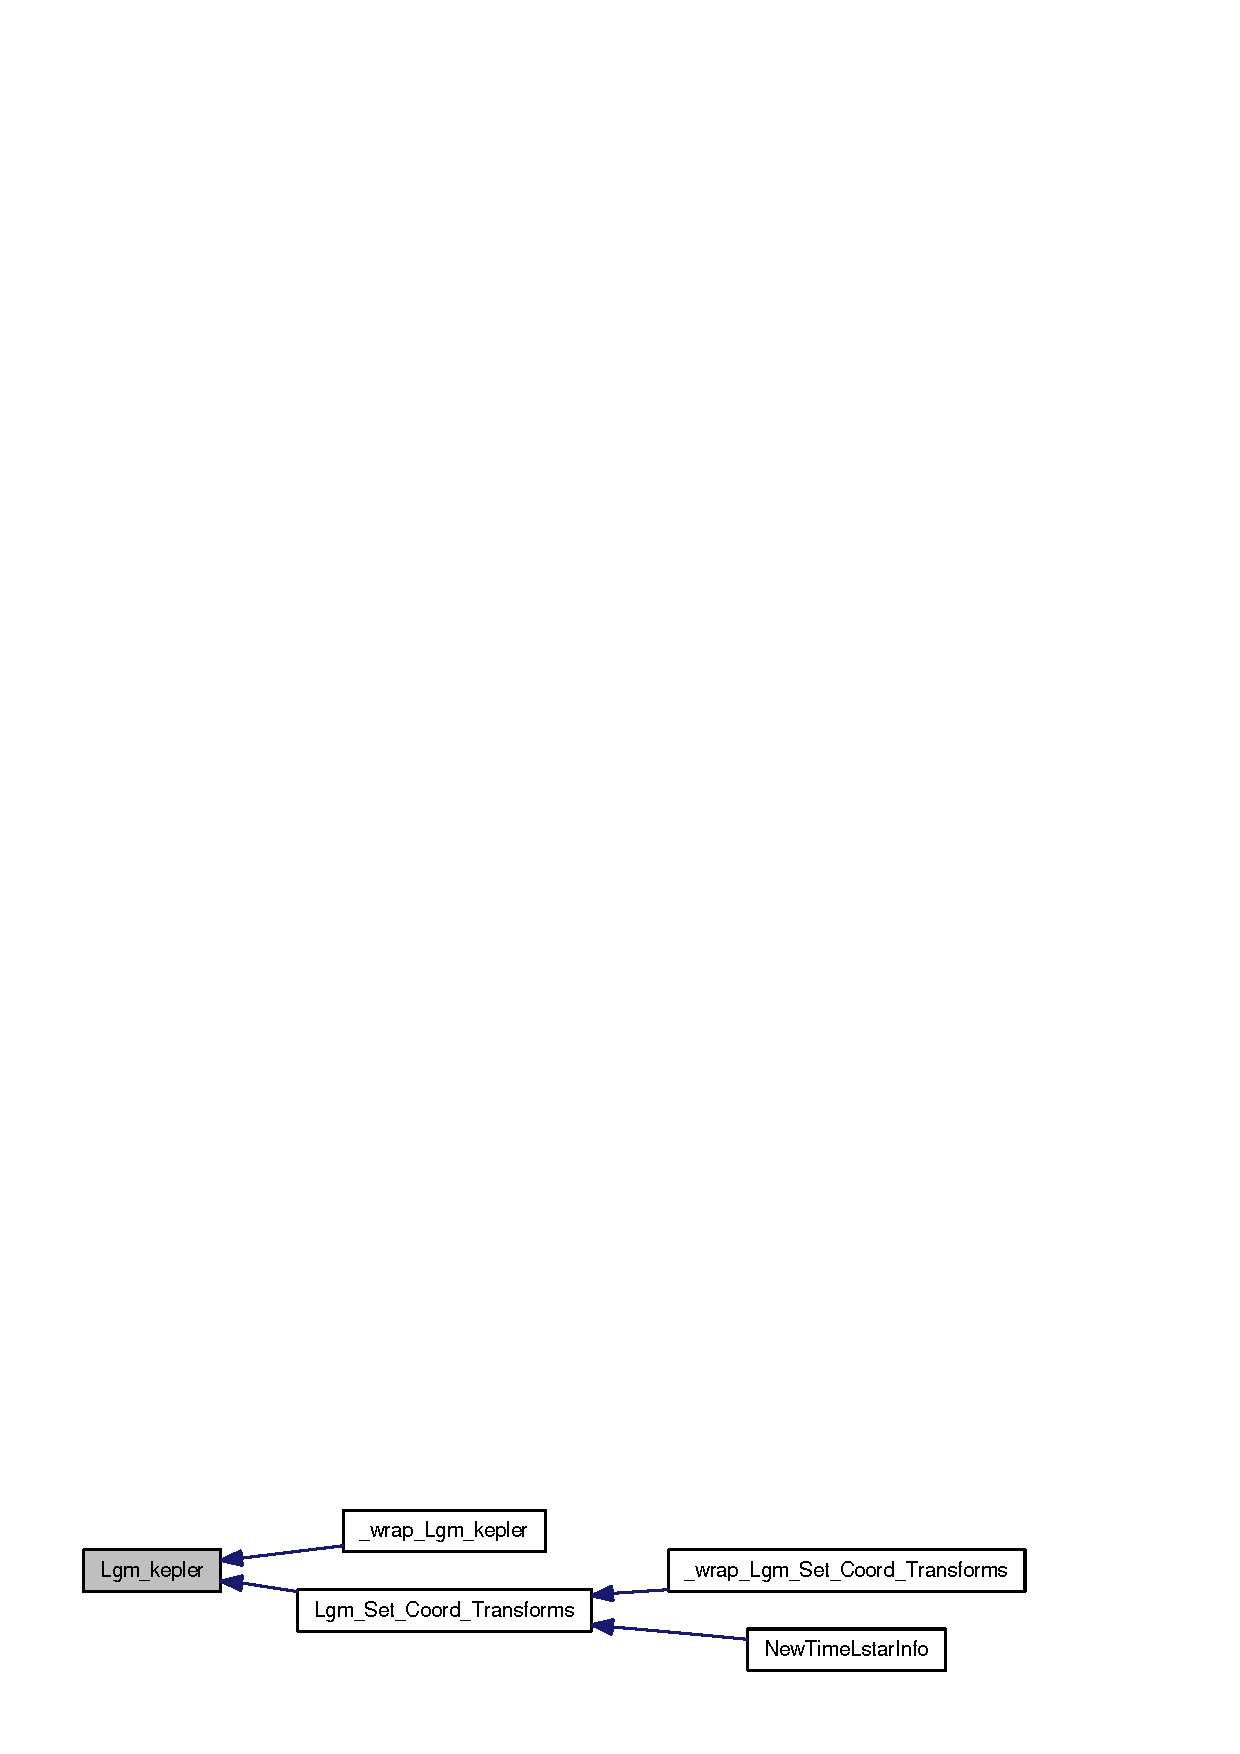
\includegraphics[width=248pt]{_lgm___c_trans_8c_59884535937bd9e67beca41c68aa0864_icgraph}
\end{center}
\end{figure}
\hypertarget{_lgm___c_trans_8c_60cb99abfbae34ae5e7a41c797dcac0e}{
\index{Lgm\_\-CTrans.c@{Lgm\_\-CTrans.c}!Lgm\_\-Set\_\-Coord\_\-Transforms@{Lgm\_\-Set\_\-Coord\_\-Transforms}}
\index{Lgm\_\-Set\_\-Coord\_\-Transforms@{Lgm\_\-Set\_\-Coord\_\-Transforms}!Lgm_CTrans.c@{Lgm\_\-CTrans.c}}
\subsubsection[{Lgm\_\-Set\_\-Coord\_\-Transforms}]{\setlength{\rightskip}{0pt plus 5cm}void Lgm\_\-Set\_\-Coord\_\-Transforms (long int {\em date}, \/  double {\em UTC}, \/  {\bf Lgm\_\-CTrans} $\ast$ {\em c})}}
\label{_lgm___c_trans_8c_60cb99abfbae34ae5e7a41c797dcac0e}




Definition at line 264 of file Lgm\_\-CTrans.c.

Here is the call graph for this function:\nopagebreak
\begin{figure}[H]
\begin{center}
\leavevmode
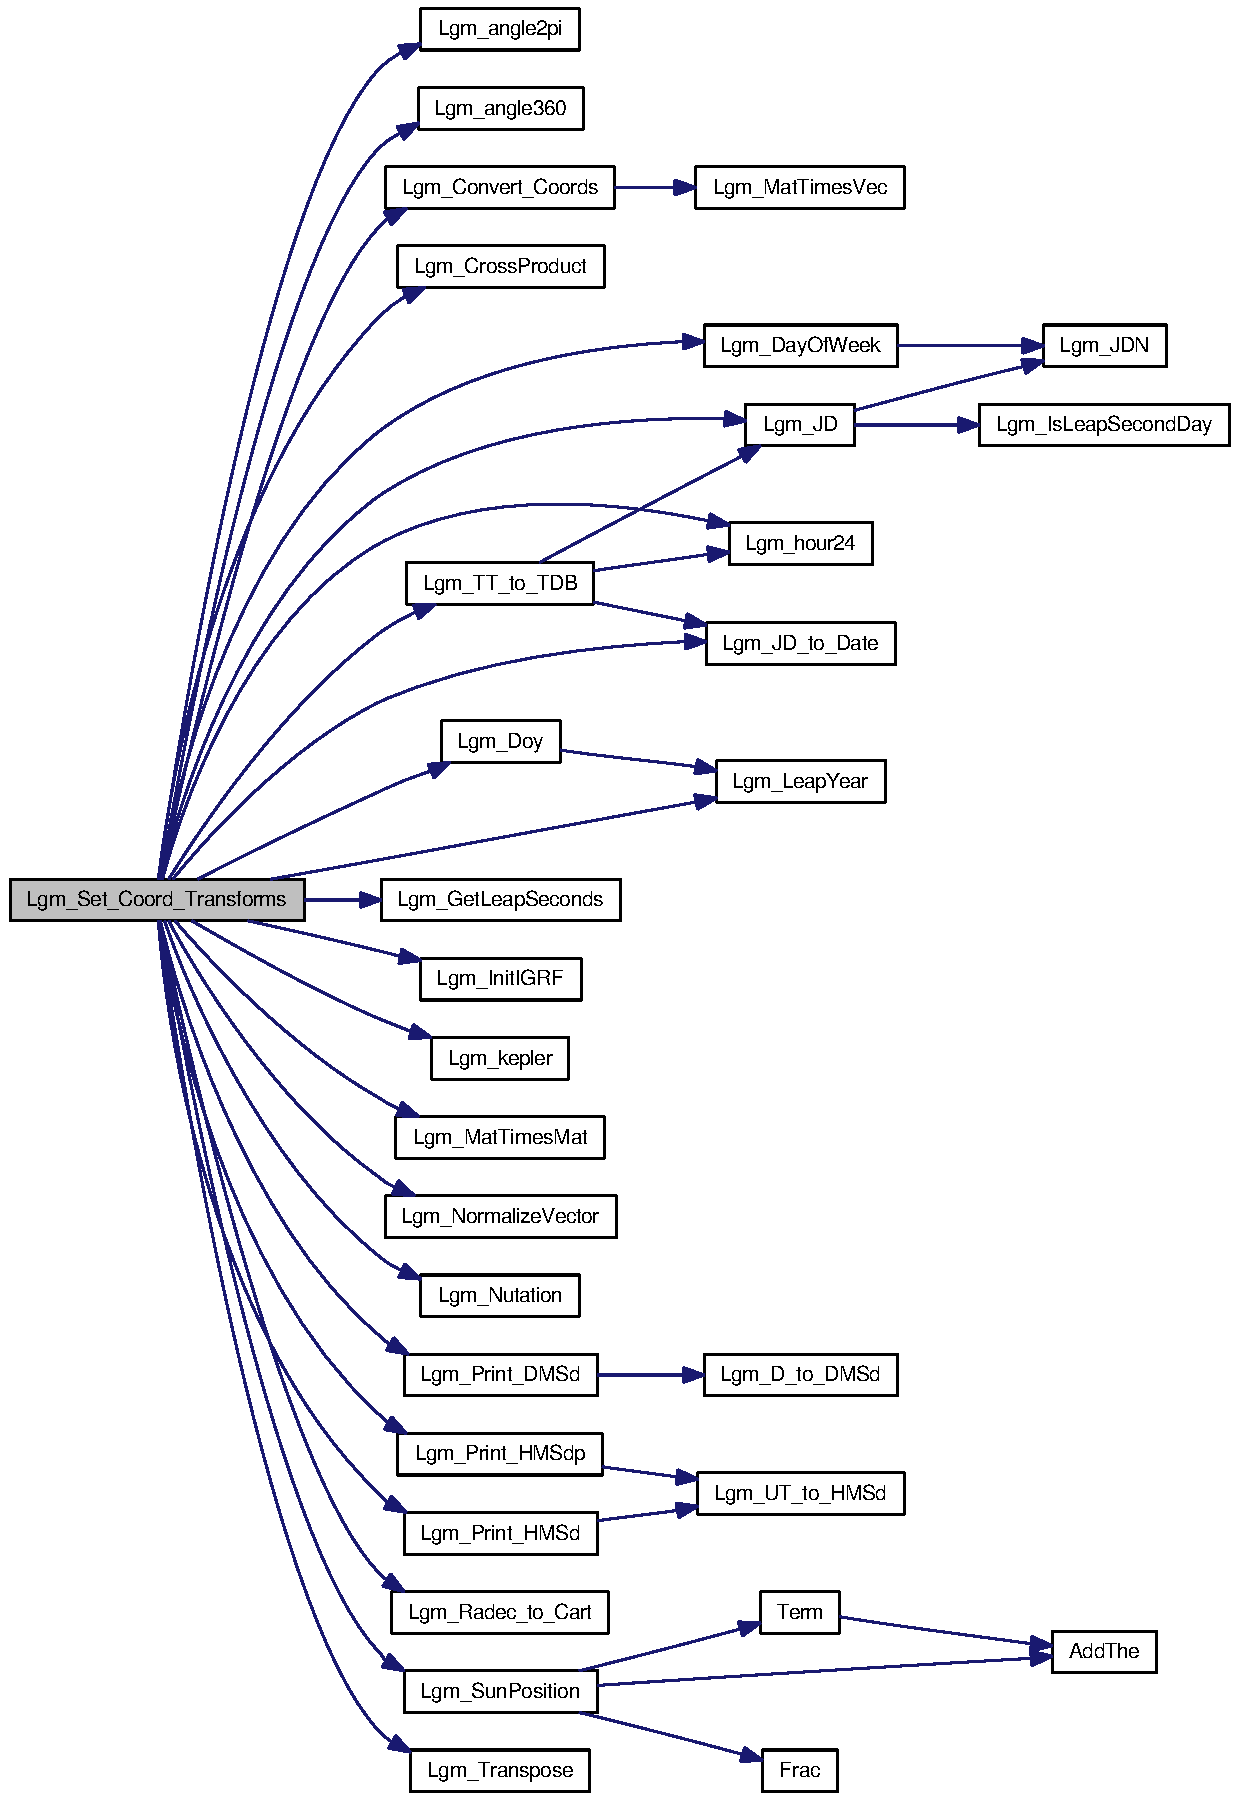
\includegraphics[width=315pt]{_lgm___c_trans_8c_60cb99abfbae34ae5e7a41c797dcac0e_cgraph}
\end{center}
\end{figure}


Here is the caller graph for this function:\nopagebreak
\begin{figure}[H]
\begin{center}
\leavevmode
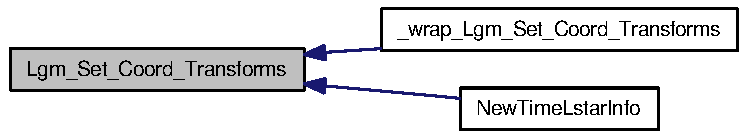
\includegraphics[width=197pt]{_lgm___c_trans_8c_60cb99abfbae34ae5e7a41c797dcac0e_icgraph}
\end{center}
\end{figure}
\hypertarget{_lgm___c_trans_8c_3975f7cfbe7332bf9b471532d496f442}{
\index{Lgm\_\-CTrans.c@{Lgm\_\-CTrans.c}!Lgm\_\-Convert\_\-Coords@{Lgm\_\-Convert\_\-Coords}}
\index{Lgm\_\-Convert\_\-Coords@{Lgm\_\-Convert\_\-Coords}!Lgm_CTrans.c@{Lgm\_\-CTrans.c}}
\subsubsection[{Lgm\_\-Convert\_\-Coords}]{\setlength{\rightskip}{0pt plus 5cm}void Lgm\_\-Convert\_\-Coords ({\bf Lgm\_\-Vector} $\ast$ {\em u}, \/  {\bf Lgm\_\-Vector} $\ast$ {\em v}, \/  int {\em flag}, \/  {\bf Lgm\_\-CTrans} $\ast$ {\em c})}}
\label{_lgm___c_trans_8c_3975f7cfbe7332bf9b471532d496f442}




Definition at line 1086 of file Lgm\_\-CTrans.c.

Here is the call graph for this function:\nopagebreak
\begin{figure}[H]
\begin{center}
\leavevmode
\includegraphics[width=145pt]{_lgm___c_trans_8c_3975f7cfbe7332bf9b471532d496f442_cgraph}
\end{center}
\end{figure}


Here is the caller graph for this function:\nopagebreak
\begin{figure}[H]
\begin{center}
\leavevmode
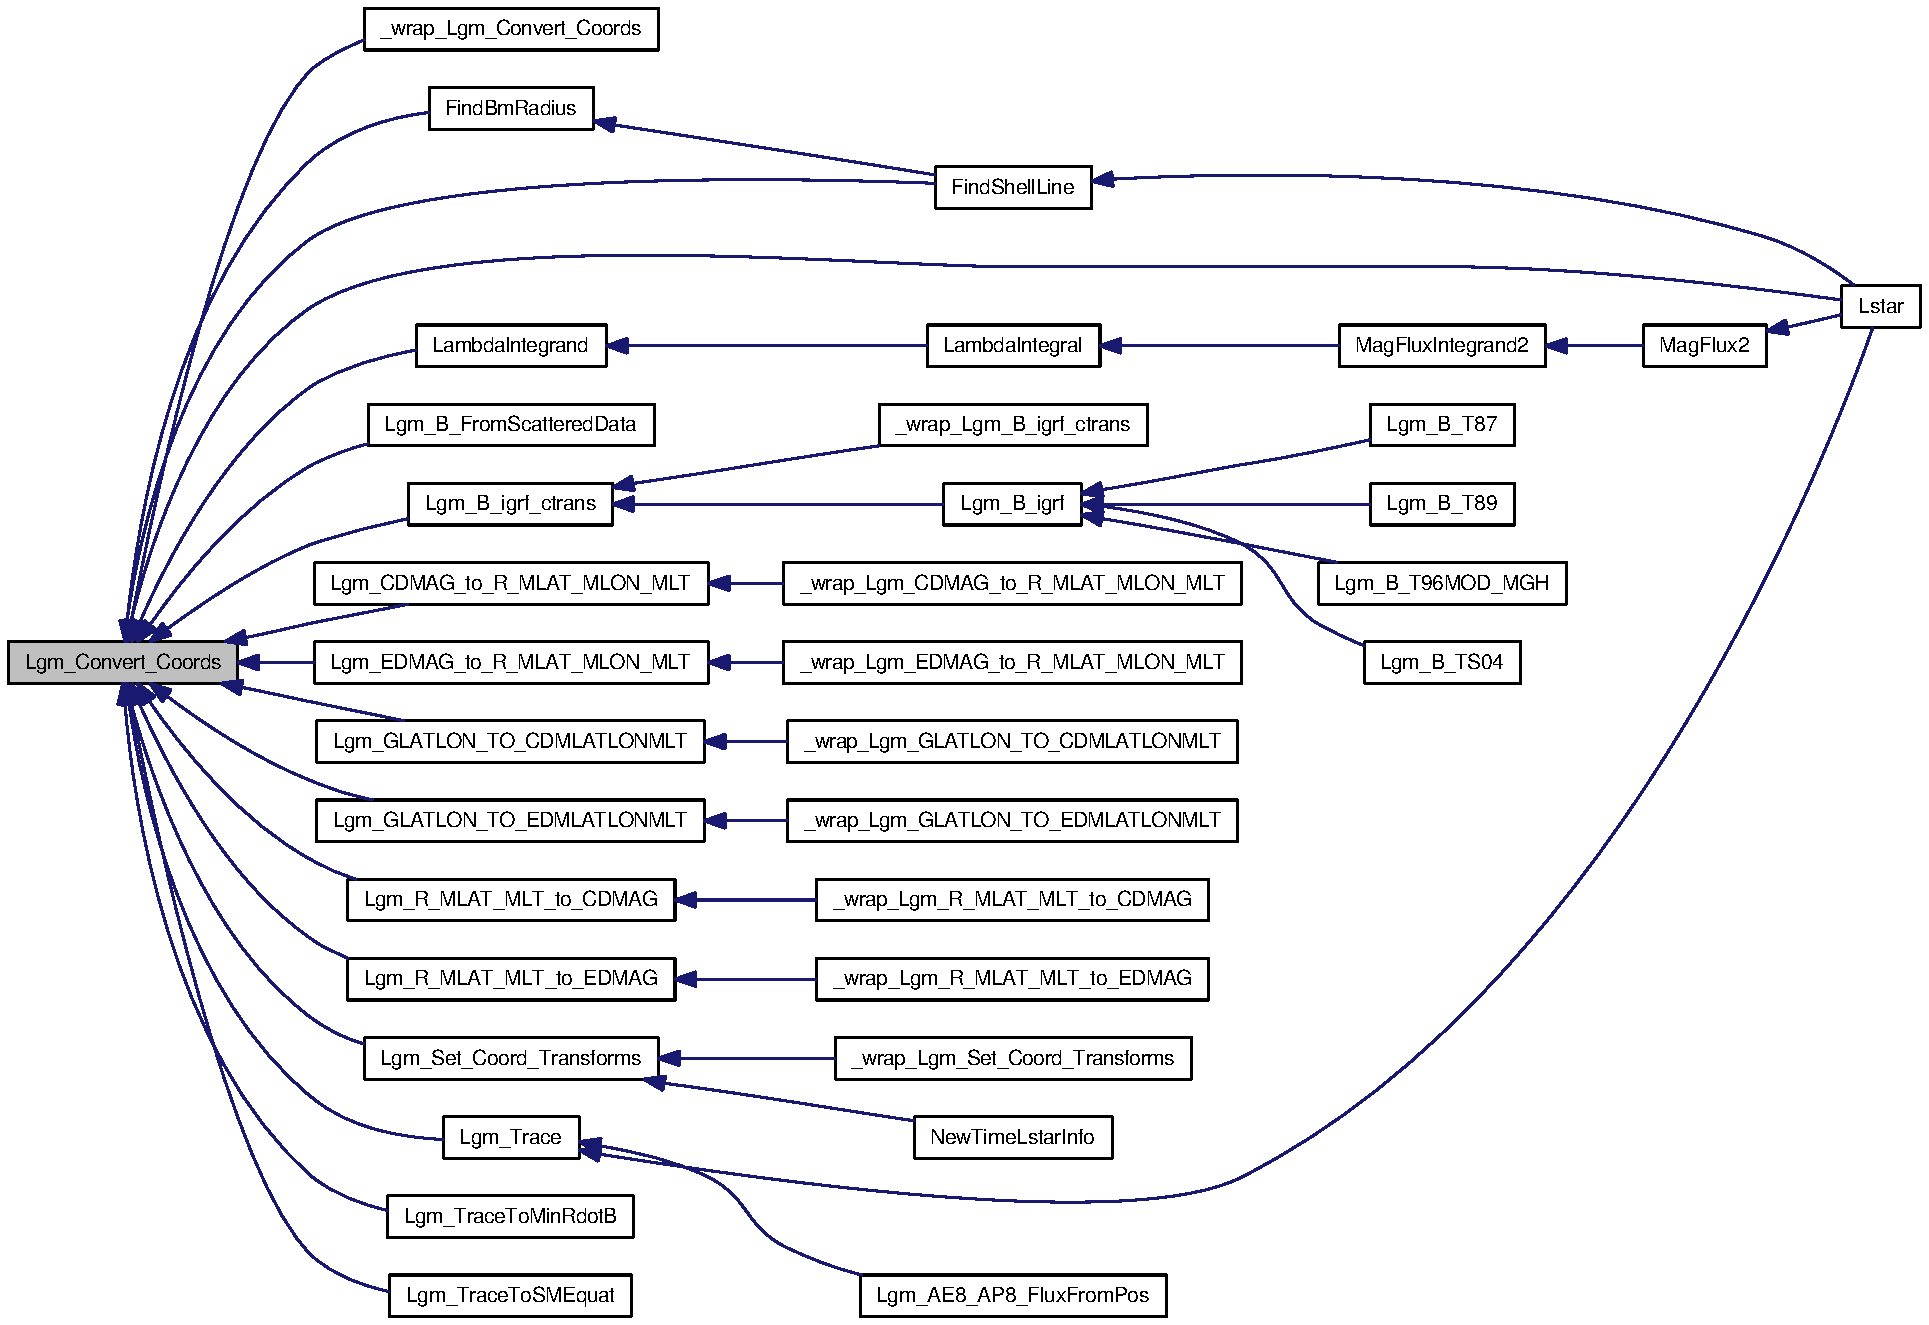
\includegraphics[width=420pt]{_lgm___c_trans_8c_3975f7cfbe7332bf9b471532d496f442_icgraph}
\end{center}
\end{figure}
\hypertarget{_lgm___c_trans_8c_765b74946e14a91f17fdb32761073682}{
\index{Lgm\_\-CTrans.c@{Lgm\_\-CTrans.c}!Lgm\_\-GEOD\_\-to\_\-WGS84@{Lgm\_\-GEOD\_\-to\_\-WGS84}}
\index{Lgm\_\-GEOD\_\-to\_\-WGS84@{Lgm\_\-GEOD\_\-to\_\-WGS84}!Lgm_CTrans.c@{Lgm\_\-CTrans.c}}
\subsubsection[{Lgm\_\-GEOD\_\-to\_\-WGS84}]{\setlength{\rightskip}{0pt plus 5cm}void Lgm\_\-GEOD\_\-to\_\-WGS84 (double {\em GeodLat}, \/  double {\em GeodLong}, \/  double {\em GeodHeight}, \/  {\bf Lgm\_\-Vector} $\ast$ {\em v})}}
\label{_lgm___c_trans_8c_765b74946e14a91f17fdb32761073682}




Definition at line 1233 of file Lgm\_\-CTrans.c.

Here is the caller graph for this function:\nopagebreak
\begin{figure}[H]
\begin{center}
\leavevmode
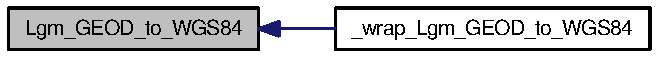
\includegraphics[width=176pt]{_lgm___c_trans_8c_765b74946e14a91f17fdb32761073682_icgraph}
\end{center}
\end{figure}
\hypertarget{_lgm___c_trans_8c_64e411cdf591772fca631d5e42fdacd3}{
\index{Lgm\_\-CTrans.c@{Lgm\_\-CTrans.c}!Lgm\_\-WGS84\_\-to\_\-GEOD@{Lgm\_\-WGS84\_\-to\_\-GEOD}}
\index{Lgm\_\-WGS84\_\-to\_\-GEOD@{Lgm\_\-WGS84\_\-to\_\-GEOD}!Lgm_CTrans.c@{Lgm\_\-CTrans.c}}
\subsubsection[{Lgm\_\-WGS84\_\-to\_\-GEOD}]{\setlength{\rightskip}{0pt plus 5cm}void Lgm\_\-WGS84\_\-to\_\-GEOD ({\bf Lgm\_\-Vector} $\ast$ {\em uin}, \/  double $\ast$ {\em GeodLat}, \/  double $\ast$ {\em GeodLong}, \/  double $\ast$ {\em GeodHeight})}}
\label{_lgm___c_trans_8c_64e411cdf591772fca631d5e42fdacd3}




Definition at line 1251 of file Lgm\_\-CTrans.c.

Here is the call graph for this function:\nopagebreak
\begin{figure}[H]
\begin{center}
\leavevmode
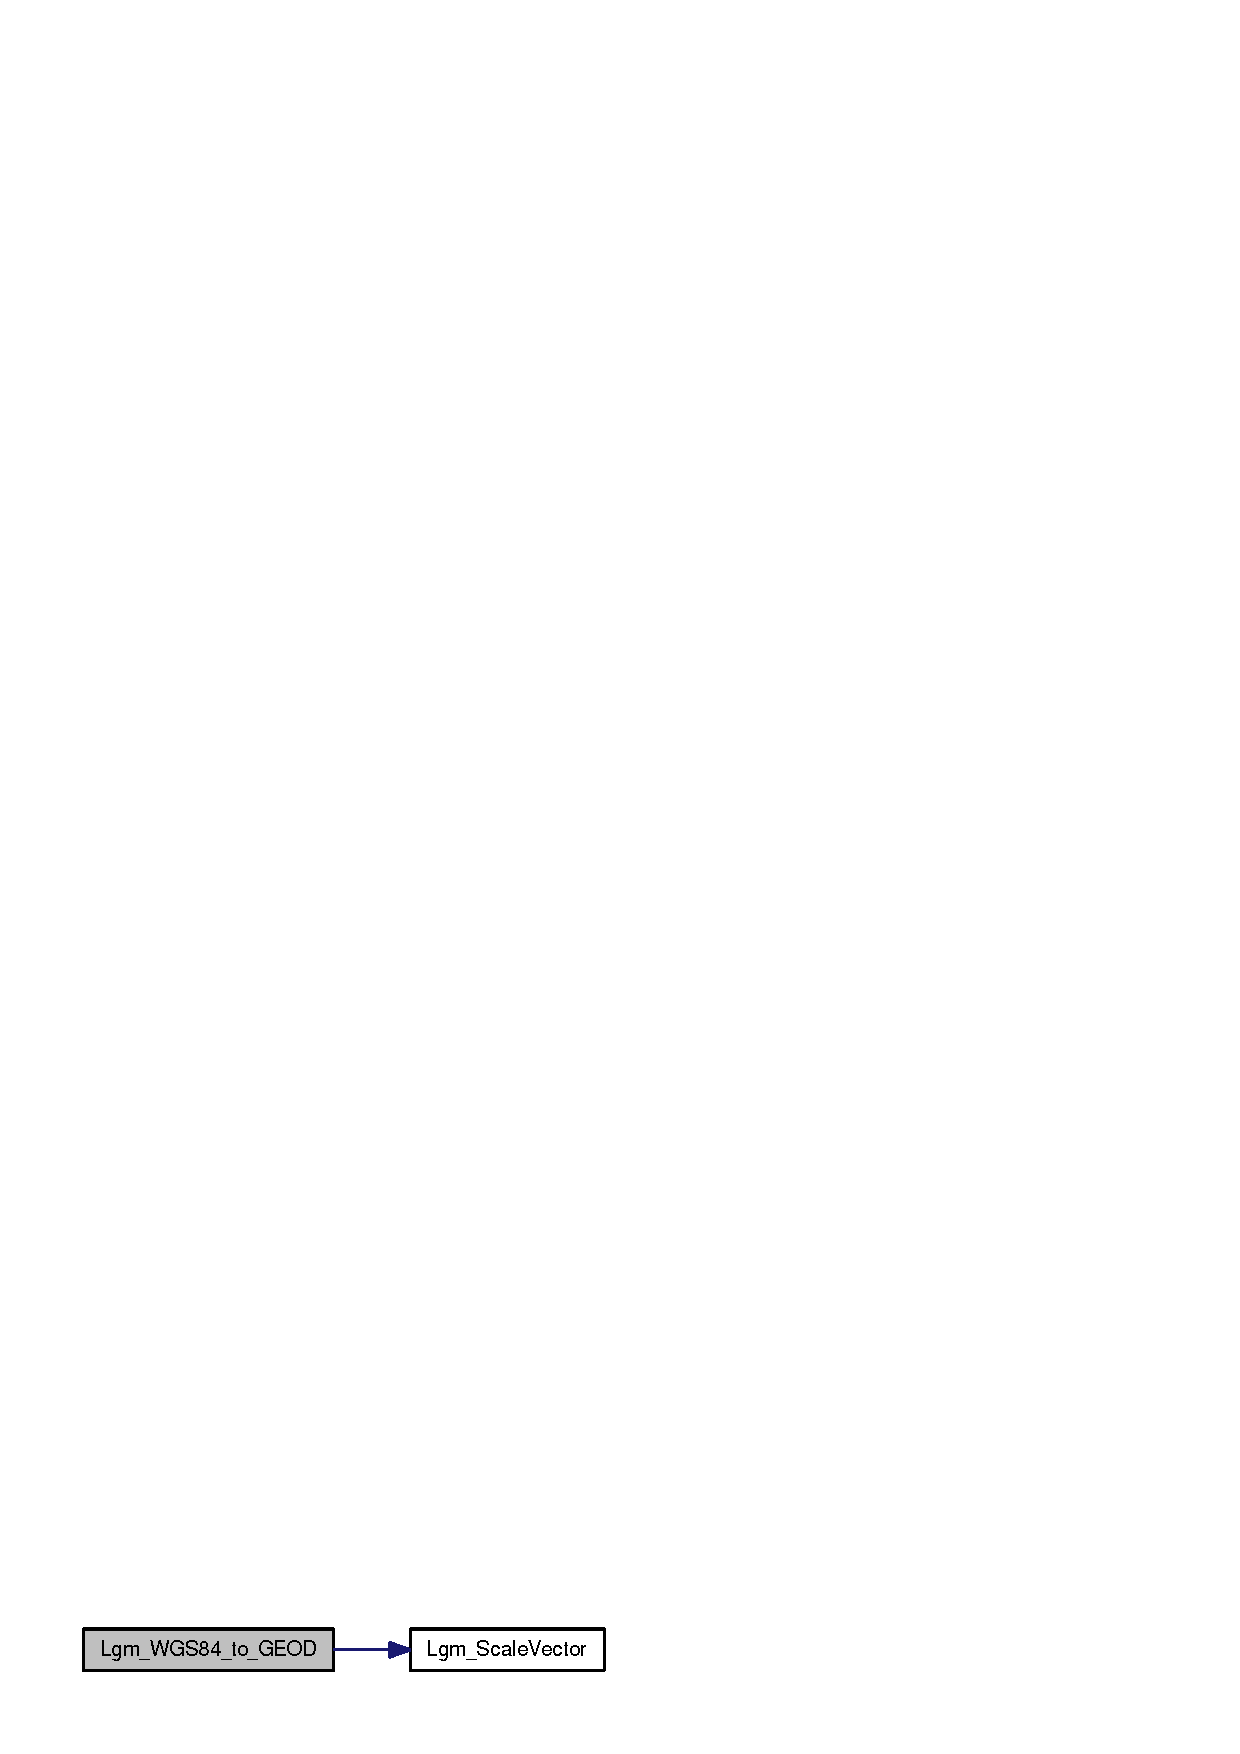
\includegraphics[width=147pt]{_lgm___c_trans_8c_64e411cdf591772fca631d5e42fdacd3_cgraph}
\end{center}
\end{figure}


Here is the caller graph for this function:\nopagebreak
\begin{figure}[H]
\begin{center}
\leavevmode
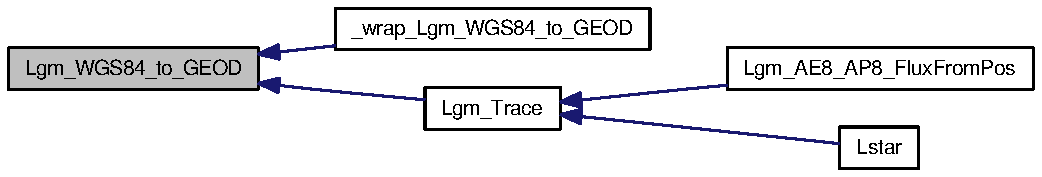
\includegraphics[width=268pt]{_lgm___c_trans_8c_64e411cdf591772fca631d5e42fdacd3_icgraph}
\end{center}
\end{figure}
\hypertarget{_lgm___c_trans_8c_323f92aef0fee19b69f4da4684fb821c}{
\index{Lgm\_\-CTrans.c@{Lgm\_\-CTrans.c}!Lgm\_\-WGS84\_\-to\_\-GeodHeight@{Lgm\_\-WGS84\_\-to\_\-GeodHeight}}
\index{Lgm\_\-WGS84\_\-to\_\-GeodHeight@{Lgm\_\-WGS84\_\-to\_\-GeodHeight}!Lgm_CTrans.c@{Lgm\_\-CTrans.c}}
\subsubsection[{Lgm\_\-WGS84\_\-to\_\-GeodHeight}]{\setlength{\rightskip}{0pt plus 5cm}void Lgm\_\-WGS84\_\-to\_\-GeodHeight ({\bf Lgm\_\-Vector} $\ast$ {\em uin}, \/  double $\ast$ {\em GeodHeight})}}
\label{_lgm___c_trans_8c_323f92aef0fee19b69f4da4684fb821c}




Definition at line 1285 of file Lgm\_\-CTrans.c.

Here is the call graph for this function:\nopagebreak
\begin{figure}[H]
\begin{center}
\leavevmode
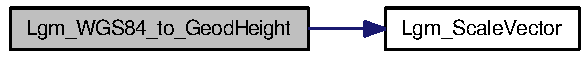
\includegraphics[width=159pt]{_lgm___c_trans_8c_323f92aef0fee19b69f4da4684fb821c_cgraph}
\end{center}
\end{figure}


Here is the caller graph for this function:\nopagebreak
\begin{figure}[H]
\begin{center}
\leavevmode
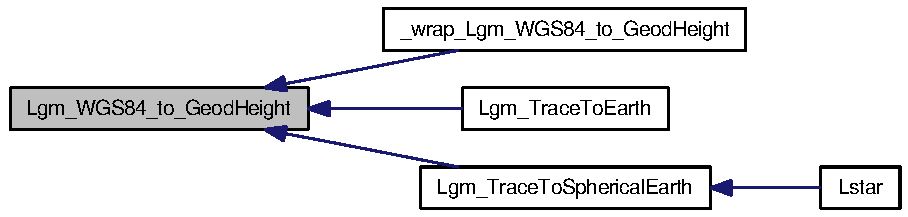
\includegraphics[width=236pt]{_lgm___c_trans_8c_323f92aef0fee19b69f4da4684fb821c_icgraph}
\end{center}
\end{figure}
\hypertarget{_lgm___c_trans_8c_4e7b063e0734746ff6af5ef5118ed8b8}{
\index{Lgm\_\-CTrans.c@{Lgm\_\-CTrans.c}!Lgm\_\-B\_\-igrf\_\-ctrans@{Lgm\_\-B\_\-igrf\_\-ctrans}}
\index{Lgm\_\-B\_\-igrf\_\-ctrans@{Lgm\_\-B\_\-igrf\_\-ctrans}!Lgm_CTrans.c@{Lgm\_\-CTrans.c}}
\subsubsection[{Lgm\_\-B\_\-igrf\_\-ctrans}]{\setlength{\rightskip}{0pt plus 5cm}void Lgm\_\-B\_\-igrf\_\-ctrans ({\bf Lgm\_\-Vector} $\ast$ {\em v}, \/  {\bf Lgm\_\-Vector} $\ast$ {\em B}, \/  {\bf Lgm\_\-CTrans} $\ast$ {\em c})}}
\label{_lgm___c_trans_8c_4e7b063e0734746ff6af5ef5118ed8b8}




Definition at line 1322 of file Lgm\_\-CTrans.c.

Here is the call graph for this function:\nopagebreak
\begin{figure}[H]
\begin{center}
\leavevmode
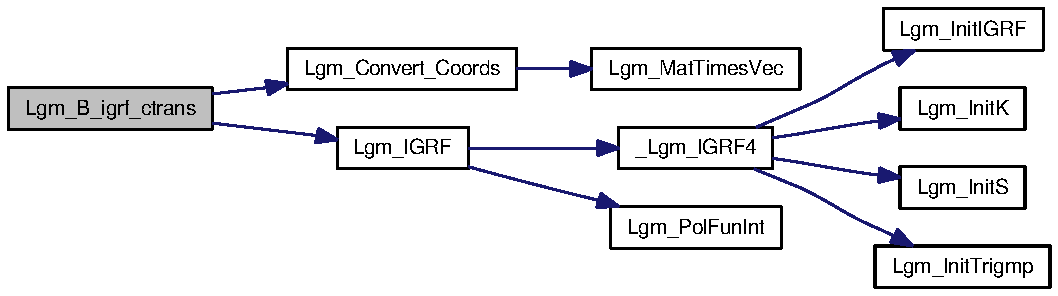
\includegraphics[width=272pt]{_lgm___c_trans_8c_4e7b063e0734746ff6af5ef5118ed8b8_cgraph}
\end{center}
\end{figure}


Here is the caller graph for this function:\nopagebreak
\begin{figure}[H]
\begin{center}
\leavevmode
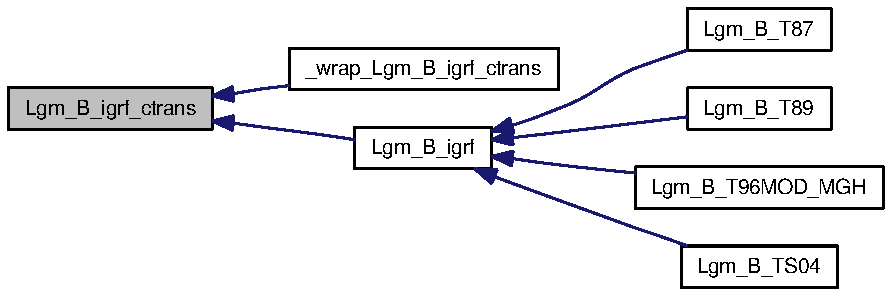
\includegraphics[width=232pt]{_lgm___c_trans_8c_4e7b063e0734746ff6af5ef5118ed8b8_icgraph}
\end{center}
\end{figure}
\hypertarget{_lgm___c_trans_8c_a23fbb09653a52bfb6e38be64231ad8d}{
\index{Lgm\_\-CTrans.c@{Lgm\_\-CTrans.c}!Lgm\_\-B\_\-cdip\_\-ctrans@{Lgm\_\-B\_\-cdip\_\-ctrans}}
\index{Lgm\_\-B\_\-cdip\_\-ctrans@{Lgm\_\-B\_\-cdip\_\-ctrans}!Lgm_CTrans.c@{Lgm\_\-CTrans.c}}
\subsubsection[{Lgm\_\-B\_\-cdip\_\-ctrans}]{\setlength{\rightskip}{0pt plus 5cm}void Lgm\_\-B\_\-cdip\_\-ctrans ({\bf Lgm\_\-Vector} $\ast$ {\em v}, \/  {\bf Lgm\_\-Vector} $\ast$ {\em B}, \/  {\bf Lgm\_\-CTrans} $\ast$ {\em c})}}
\label{_lgm___c_trans_8c_a23fbb09653a52bfb6e38be64231ad8d}




Definition at line 1374 of file Lgm\_\-CTrans.c.

Here is the caller graph for this function:\nopagebreak
\begin{figure}[H]
\begin{center}
\leavevmode
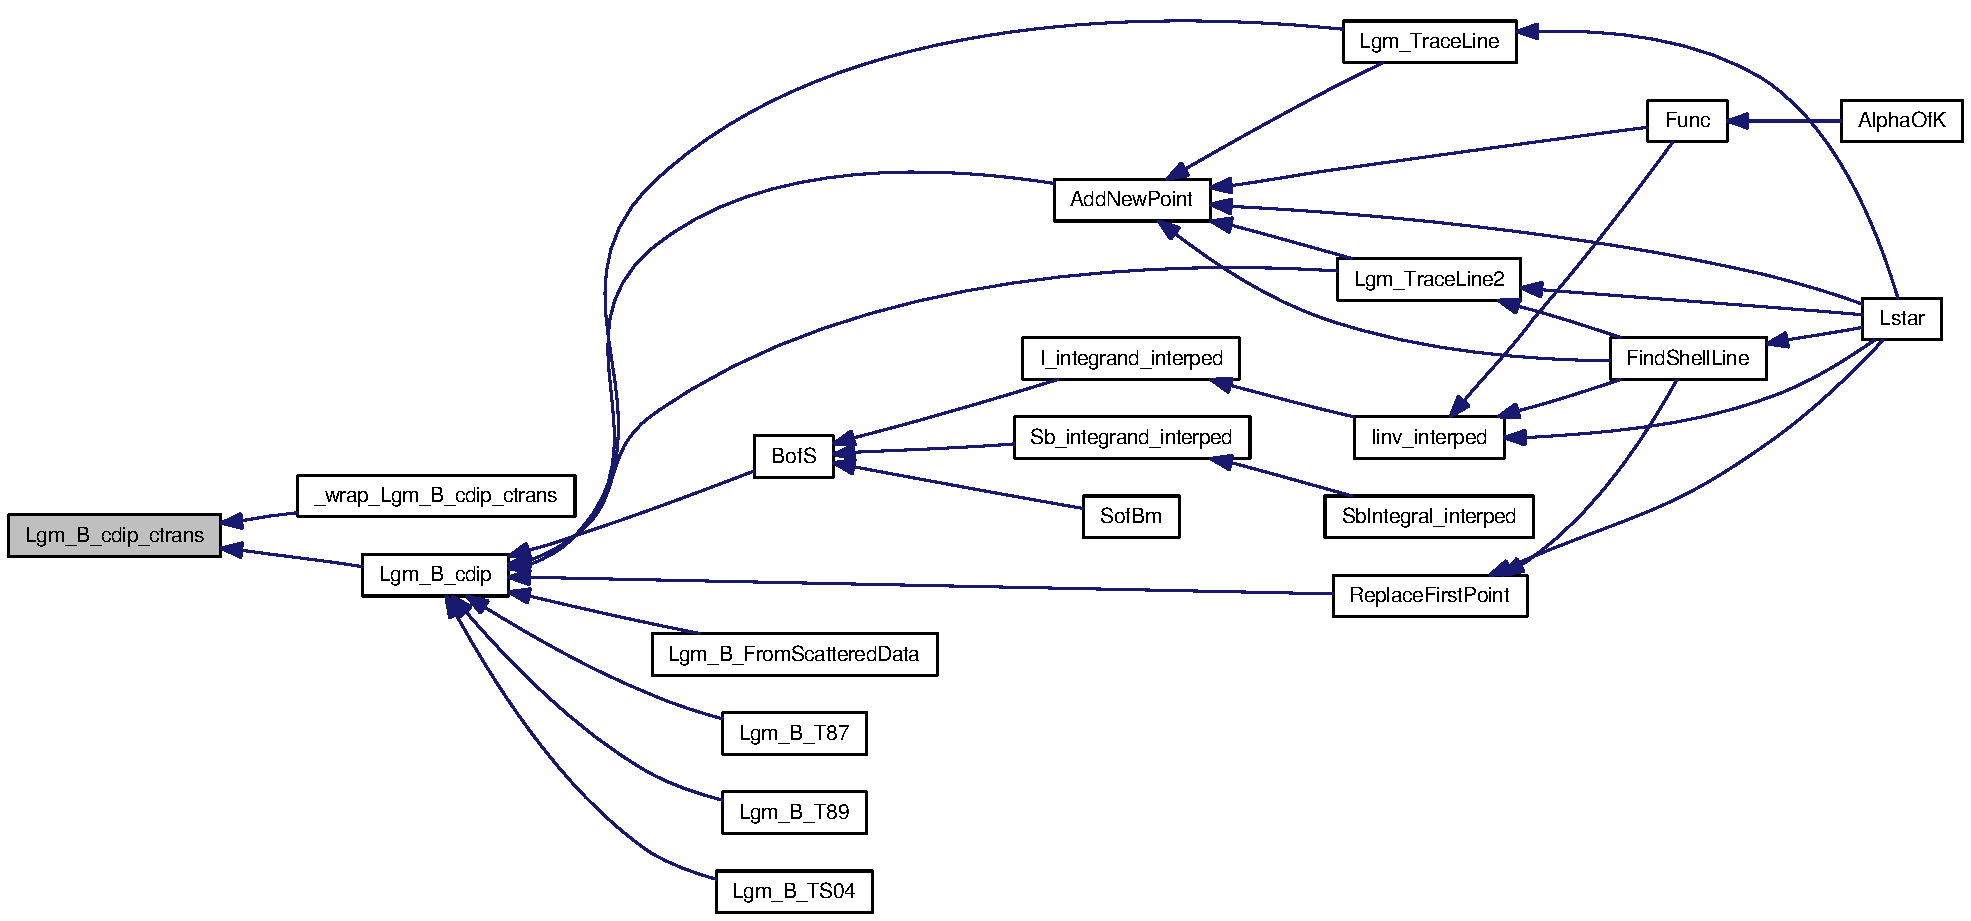
\includegraphics[width=420pt]{_lgm___c_trans_8c_a23fbb09653a52bfb6e38be64231ad8d_icgraph}
\end{center}
\end{figure}
\hypertarget{_lgm___c_trans_8c_5302ef2d070d2764b911aac4cbd2f4f0}{
\index{Lgm\_\-CTrans.c@{Lgm\_\-CTrans.c}!Lgm\_\-B\_\-edip\_\-ctrans@{Lgm\_\-B\_\-edip\_\-ctrans}}
\index{Lgm\_\-B\_\-edip\_\-ctrans@{Lgm\_\-B\_\-edip\_\-ctrans}!Lgm_CTrans.c@{Lgm\_\-CTrans.c}}
\subsubsection[{Lgm\_\-B\_\-edip\_\-ctrans}]{\setlength{\rightskip}{0pt plus 5cm}void Lgm\_\-B\_\-edip\_\-ctrans ({\bf Lgm\_\-Vector} $\ast$ {\em v}, \/  {\bf Lgm\_\-Vector} $\ast$ {\em B}, \/  {\bf Lgm\_\-CTrans} $\ast$ {\em c})}}
\label{_lgm___c_trans_8c_5302ef2d070d2764b911aac4cbd2f4f0}




Definition at line 1435 of file Lgm\_\-CTrans.c.

Here is the caller graph for this function:\nopagebreak
\begin{figure}[H]
\begin{center}
\leavevmode
\includegraphics[width=214pt]{_lgm___c_trans_8c_5302ef2d070d2764b911aac4cbd2f4f0_icgraph}
\end{center}
\end{figure}
\hypertarget{_lgm___c_trans_8c_8235053e9b85c2b8573f4631df5406a1}{
\index{Lgm\_\-CTrans.c@{Lgm\_\-CTrans.c}!Lgm\_\-jd\_\-to\_\-ymdh@{Lgm\_\-jd\_\-to\_\-ymdh}}
\index{Lgm\_\-jd\_\-to\_\-ymdh@{Lgm\_\-jd\_\-to\_\-ymdh}!Lgm_CTrans.c@{Lgm\_\-CTrans.c}}
\subsubsection[{Lgm\_\-jd\_\-to\_\-ymdh}]{\setlength{\rightskip}{0pt plus 5cm}void Lgm\_\-jd\_\-to\_\-ymdh (double {\em JD}, \/  long int $\ast$ {\em Date}, \/  int $\ast$ {\em year}, \/  int $\ast$ {\em month}, \/  int $\ast$ {\em day}, \/  double $\ast$ {\em UT})}}
\label{_lgm___c_trans_8c_8235053e9b85c2b8573f4631df5406a1}




Definition at line 1509 of file Lgm\_\-CTrans.c.

Here is the caller graph for this function:\nopagebreak
\begin{figure}[H]
\begin{center}
\leavevmode
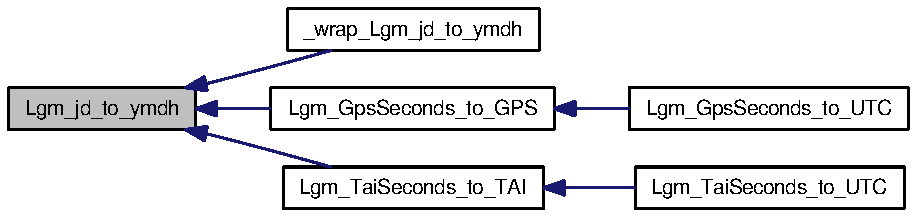
\includegraphics[width=238pt]{_lgm___c_trans_8c_8235053e9b85c2b8573f4631df5406a1_icgraph}
\end{center}
\end{figure}
\hypertarget{_lgm___c_trans_8c_18027f421b92398b5b8c53915f340759}{
\index{Lgm\_\-CTrans.c@{Lgm\_\-CTrans.c}!Lgm\_\-mjd\_\-to\_\-ymdh@{Lgm\_\-mjd\_\-to\_\-ymdh}}
\index{Lgm\_\-mjd\_\-to\_\-ymdh@{Lgm\_\-mjd\_\-to\_\-ymdh}!Lgm_CTrans.c@{Lgm\_\-CTrans.c}}
\subsubsection[{Lgm\_\-mjd\_\-to\_\-ymdh}]{\setlength{\rightskip}{0pt plus 5cm}void Lgm\_\-mjd\_\-to\_\-ymdh (double {\em MJD}, \/  long int $\ast$ {\em Date}, \/  int $\ast$ {\em year}, \/  int $\ast$ {\em month}, \/  int $\ast$ {\em day}, \/  double $\ast$ {\em UT})}}
\label{_lgm___c_trans_8c_18027f421b92398b5b8c53915f340759}




Definition at line 1551 of file Lgm\_\-CTrans.c.

Here is the call graph for this function:\nopagebreak
\begin{figure}[H]
\begin{center}
\leavevmode
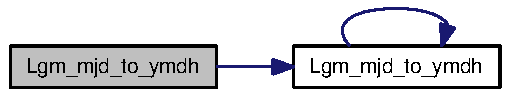
\includegraphics[width=140pt]{_lgm___c_trans_8c_18027f421b92398b5b8c53915f340759_cgraph}
\end{center}
\end{figure}


Here is the caller graph for this function:\nopagebreak
\begin{figure}[H]
\begin{center}
\leavevmode
\includegraphics[width=155pt]{_lgm___c_trans_8c_18027f421b92398b5b8c53915f340759_icgraph}
\end{center}
\end{figure}
\hypertarget{_lgm___c_trans_8c_66b28744847e26256778562fd41d07fb}{
\index{Lgm\_\-CTrans.c@{Lgm\_\-CTrans.c}!Lgm\_\-UT\_\-to\_\-hmsms@{Lgm\_\-UT\_\-to\_\-hmsms}}
\index{Lgm\_\-UT\_\-to\_\-hmsms@{Lgm\_\-UT\_\-to\_\-hmsms}!Lgm_CTrans.c@{Lgm\_\-CTrans.c}}
\subsubsection[{Lgm\_\-UT\_\-to\_\-hmsms}]{\setlength{\rightskip}{0pt plus 5cm}void Lgm\_\-UT\_\-to\_\-hmsms (double {\em UT}, \/  int $\ast$ {\em Hour}, \/  int $\ast$ {\em Min}, \/  int $\ast$ {\em Sec}, \/  int $\ast$ {\em MilliSec})}}
\label{_lgm___c_trans_8c_66b28744847e26256778562fd41d07fb}




Definition at line 1560 of file Lgm\_\-CTrans.c.

Here is the caller graph for this function:\nopagebreak
\begin{figure}[H]
\begin{center}
\leavevmode
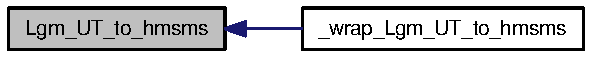
\includegraphics[width=160pt]{_lgm___c_trans_8c_66b28744847e26256778562fd41d07fb_icgraph}
\end{center}
\end{figure}
\hypertarget{_lgm___c_trans_8c_4c5eb958c42764eb7c98c2209a191d6e}{
\index{Lgm\_\-CTrans.c@{Lgm\_\-CTrans.c}!Lgm\_\-UT\_\-to\_\-HMS@{Lgm\_\-UT\_\-to\_\-HMS}}
\index{Lgm\_\-UT\_\-to\_\-HMS@{Lgm\_\-UT\_\-to\_\-HMS}!Lgm_CTrans.c@{Lgm\_\-CTrans.c}}
\subsubsection[{Lgm\_\-UT\_\-to\_\-HMS}]{\setlength{\rightskip}{0pt plus 5cm}void Lgm\_\-UT\_\-to\_\-HMS (double {\em UT}, \/  int $\ast$ {\em HH}, \/  int $\ast$ {\em MM}, \/  int $\ast$ {\em SS})}}
\label{_lgm___c_trans_8c_4c5eb958c42764eb7c98c2209a191d6e}




Definition at line 1587 of file Lgm\_\-CTrans.c.

Here is the caller graph for this function:\nopagebreak
\begin{figure}[H]
\begin{center}
\leavevmode
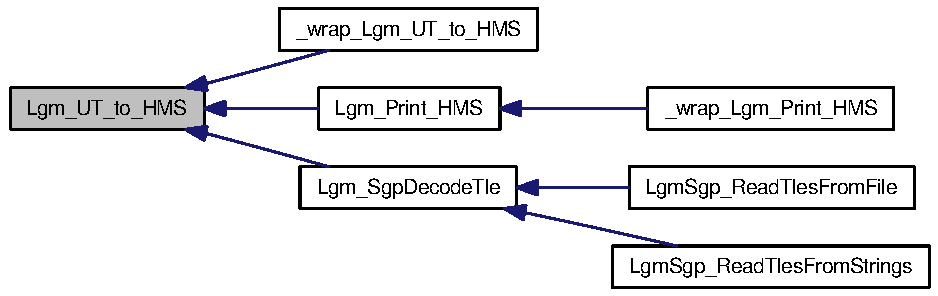
\includegraphics[width=243pt]{_lgm___c_trans_8c_4c5eb958c42764eb7c98c2209a191d6e_icgraph}
\end{center}
\end{figure}
\hypertarget{_lgm___c_trans_8c_df736dd325580fae9f0bd5fde0fab40e}{
\index{Lgm\_\-CTrans.c@{Lgm\_\-CTrans.c}!Lgm\_\-UT\_\-to\_\-HMSd@{Lgm\_\-UT\_\-to\_\-HMSd}}
\index{Lgm\_\-UT\_\-to\_\-HMSd@{Lgm\_\-UT\_\-to\_\-HMSd}!Lgm_CTrans.c@{Lgm\_\-CTrans.c}}
\subsubsection[{Lgm\_\-UT\_\-to\_\-HMSd}]{\setlength{\rightskip}{0pt plus 5cm}void Lgm\_\-UT\_\-to\_\-HMSd (double {\em UT}, \/  int $\ast$ {\em sgn}, \/  int $\ast$ {\em HH}, \/  int $\ast$ {\em MM}, \/  double $\ast$ {\em SS})}}
\label{_lgm___c_trans_8c_df736dd325580fae9f0bd5fde0fab40e}




Definition at line 1609 of file Lgm\_\-CTrans.c.

Here is the caller graph for this function:\nopagebreak
\begin{figure}[H]
\begin{center}
\leavevmode
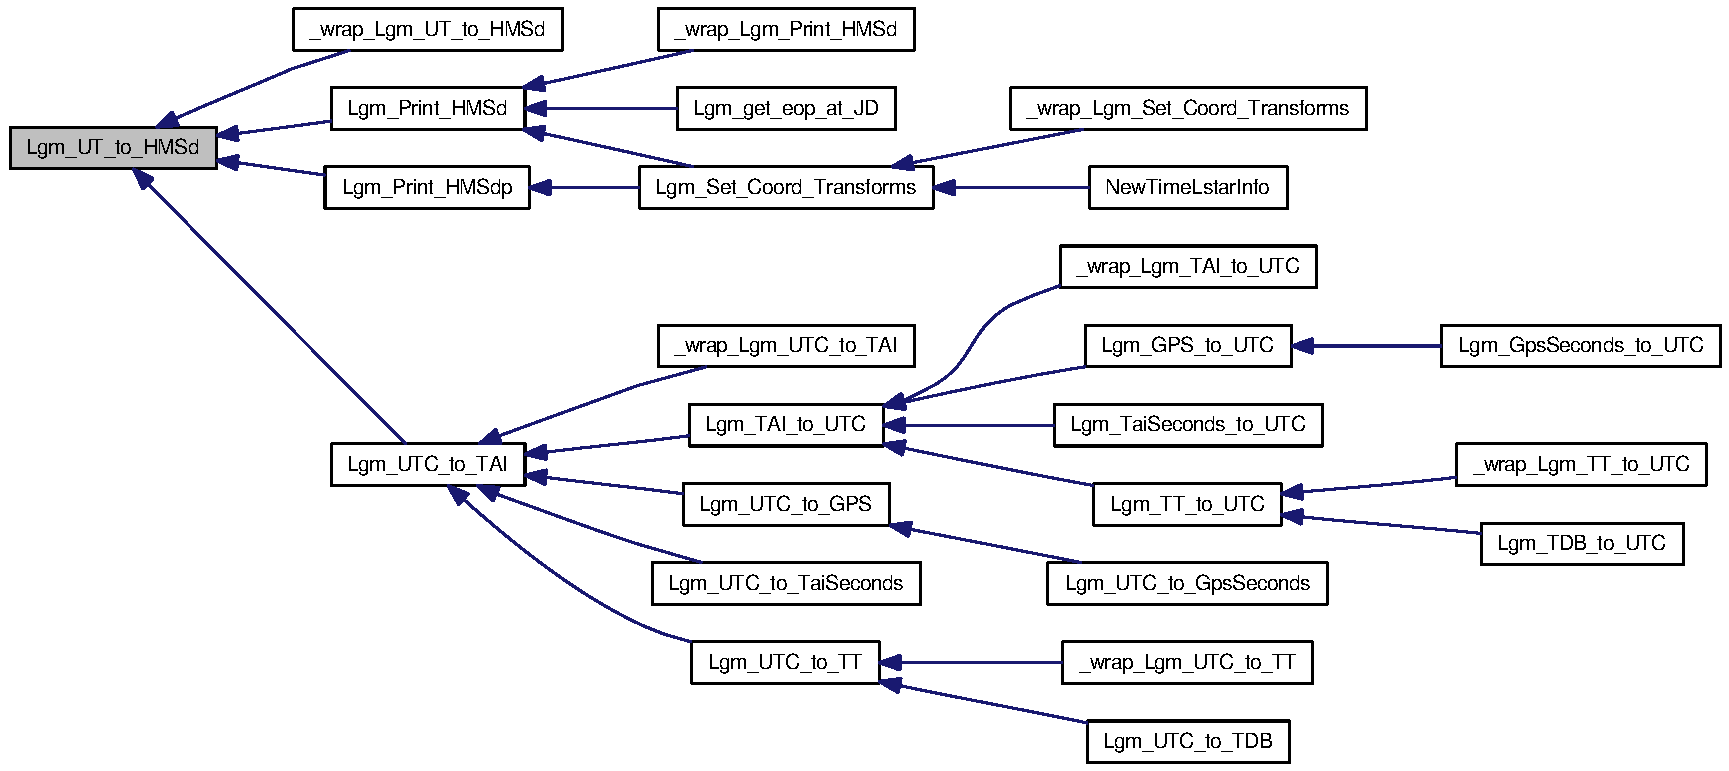
\includegraphics[width=420pt]{_lgm___c_trans_8c_df736dd325580fae9f0bd5fde0fab40e_icgraph}
\end{center}
\end{figure}
\hypertarget{_lgm___c_trans_8c_44f52ee0cf2a11d21329cc7d65448840}{
\index{Lgm\_\-CTrans.c@{Lgm\_\-CTrans.c}!Lgm\_\-D\_\-to\_\-DMS@{Lgm\_\-D\_\-to\_\-DMS}}
\index{Lgm\_\-D\_\-to\_\-DMS@{Lgm\_\-D\_\-to\_\-DMS}!Lgm_CTrans.c@{Lgm\_\-CTrans.c}}
\subsubsection[{Lgm\_\-D\_\-to\_\-DMS}]{\setlength{\rightskip}{0pt plus 5cm}void Lgm\_\-D\_\-to\_\-DMS (double {\em D}, \/  int $\ast$ {\em DD}, \/  int $\ast$ {\em MM}, \/  int $\ast$ {\em SS})}}
\label{_lgm___c_trans_8c_44f52ee0cf2a11d21329cc7d65448840}




Definition at line 1645 of file Lgm\_\-CTrans.c.

Here is the caller graph for this function:\nopagebreak
\begin{figure}[H]
\begin{center}
\leavevmode
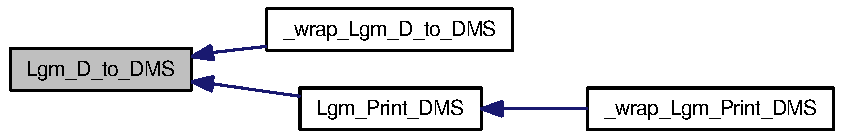
\includegraphics[width=220pt]{_lgm___c_trans_8c_44f52ee0cf2a11d21329cc7d65448840_icgraph}
\end{center}
\end{figure}
\hypertarget{_lgm___c_trans_8c_0366f317f96ffed4e998ce1551d5c190}{
\index{Lgm\_\-CTrans.c@{Lgm\_\-CTrans.c}!Lgm\_\-D\_\-to\_\-DMSd@{Lgm\_\-D\_\-to\_\-DMSd}}
\index{Lgm\_\-D\_\-to\_\-DMSd@{Lgm\_\-D\_\-to\_\-DMSd}!Lgm_CTrans.c@{Lgm\_\-CTrans.c}}
\subsubsection[{Lgm\_\-D\_\-to\_\-DMSd}]{\setlength{\rightskip}{0pt plus 5cm}void Lgm\_\-D\_\-to\_\-DMSd (double {\em D}, \/  int $\ast$ {\em sgn}, \/  int $\ast$ {\em DD}, \/  int $\ast$ {\em MM}, \/  double $\ast$ {\em SS})}}
\label{_lgm___c_trans_8c_0366f317f96ffed4e998ce1551d5c190}




Definition at line 1681 of file Lgm\_\-CTrans.c.

Here is the caller graph for this function:\nopagebreak
\begin{figure}[H]
\begin{center}
\leavevmode
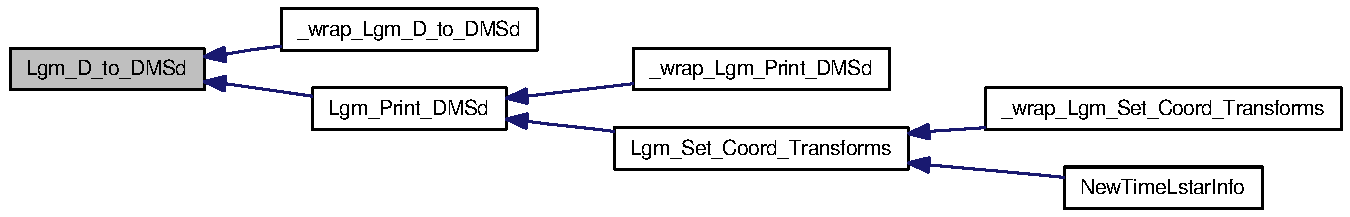
\includegraphics[width=342pt]{_lgm___c_trans_8c_0366f317f96ffed4e998ce1551d5c190_icgraph}
\end{center}
\end{figure}
\hypertarget{_lgm___c_trans_8c_8282c3981409facddb1146c8a38a6473}{
\index{Lgm\_\-CTrans.c@{Lgm\_\-CTrans.c}!Lgm\_\-GetCurrentJD@{Lgm\_\-GetCurrentJD}}
\index{Lgm\_\-GetCurrentJD@{Lgm\_\-GetCurrentJD}!Lgm_CTrans.c@{Lgm\_\-CTrans.c}}
\subsubsection[{Lgm\_\-GetCurrentJD}]{\setlength{\rightskip}{0pt plus 5cm}double Lgm\_\-GetCurrentJD ({\bf Lgm\_\-CTrans} $\ast$ {\em c})}}
\label{_lgm___c_trans_8c_8282c3981409facddb1146c8a38a6473}




Definition at line 1699 of file Lgm\_\-CTrans.c.

Here is the call graph for this function:\nopagebreak
\begin{figure}[H]
\begin{center}
\leavevmode
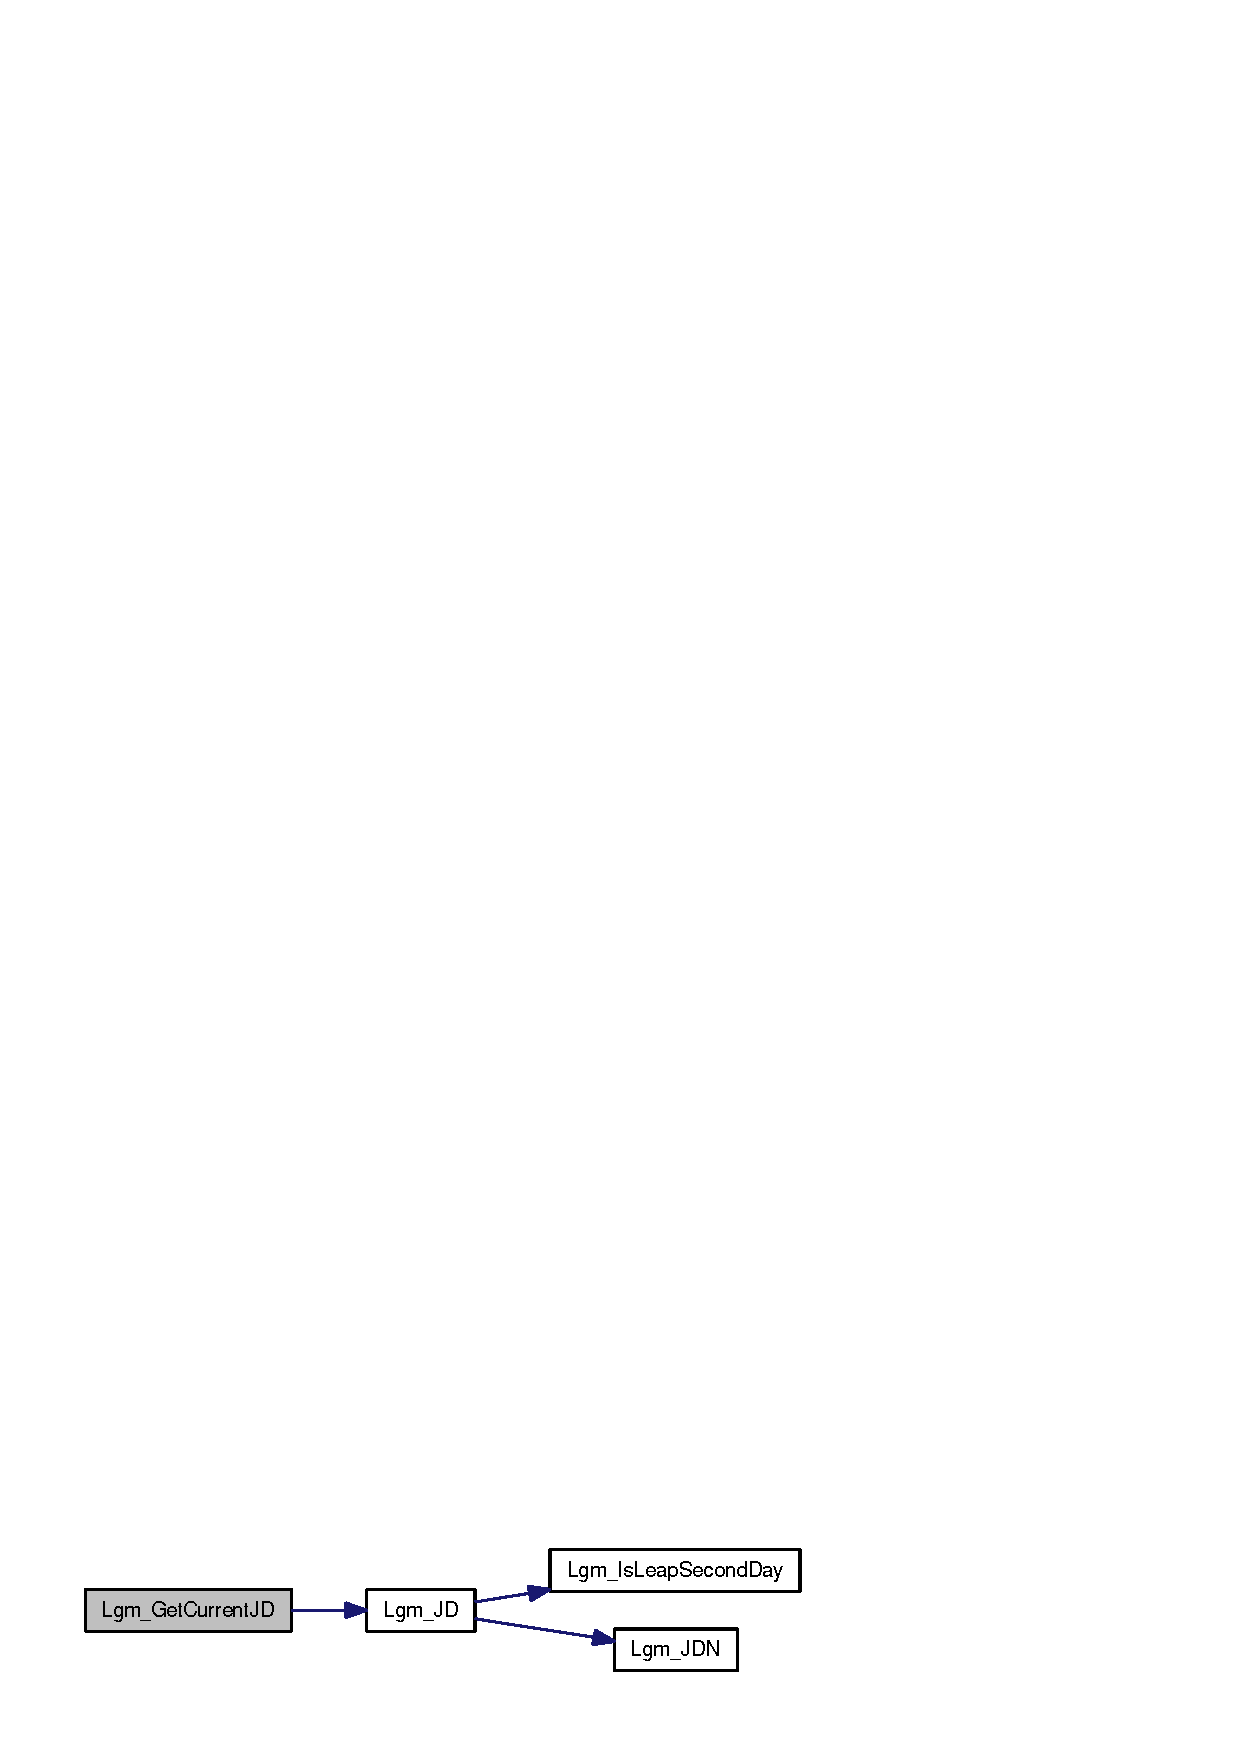
\includegraphics[width=194pt]{_lgm___c_trans_8c_8282c3981409facddb1146c8a38a6473_cgraph}
\end{center}
\end{figure}


Here is the caller graph for this function:\nopagebreak
\begin{figure}[H]
\begin{center}
\leavevmode
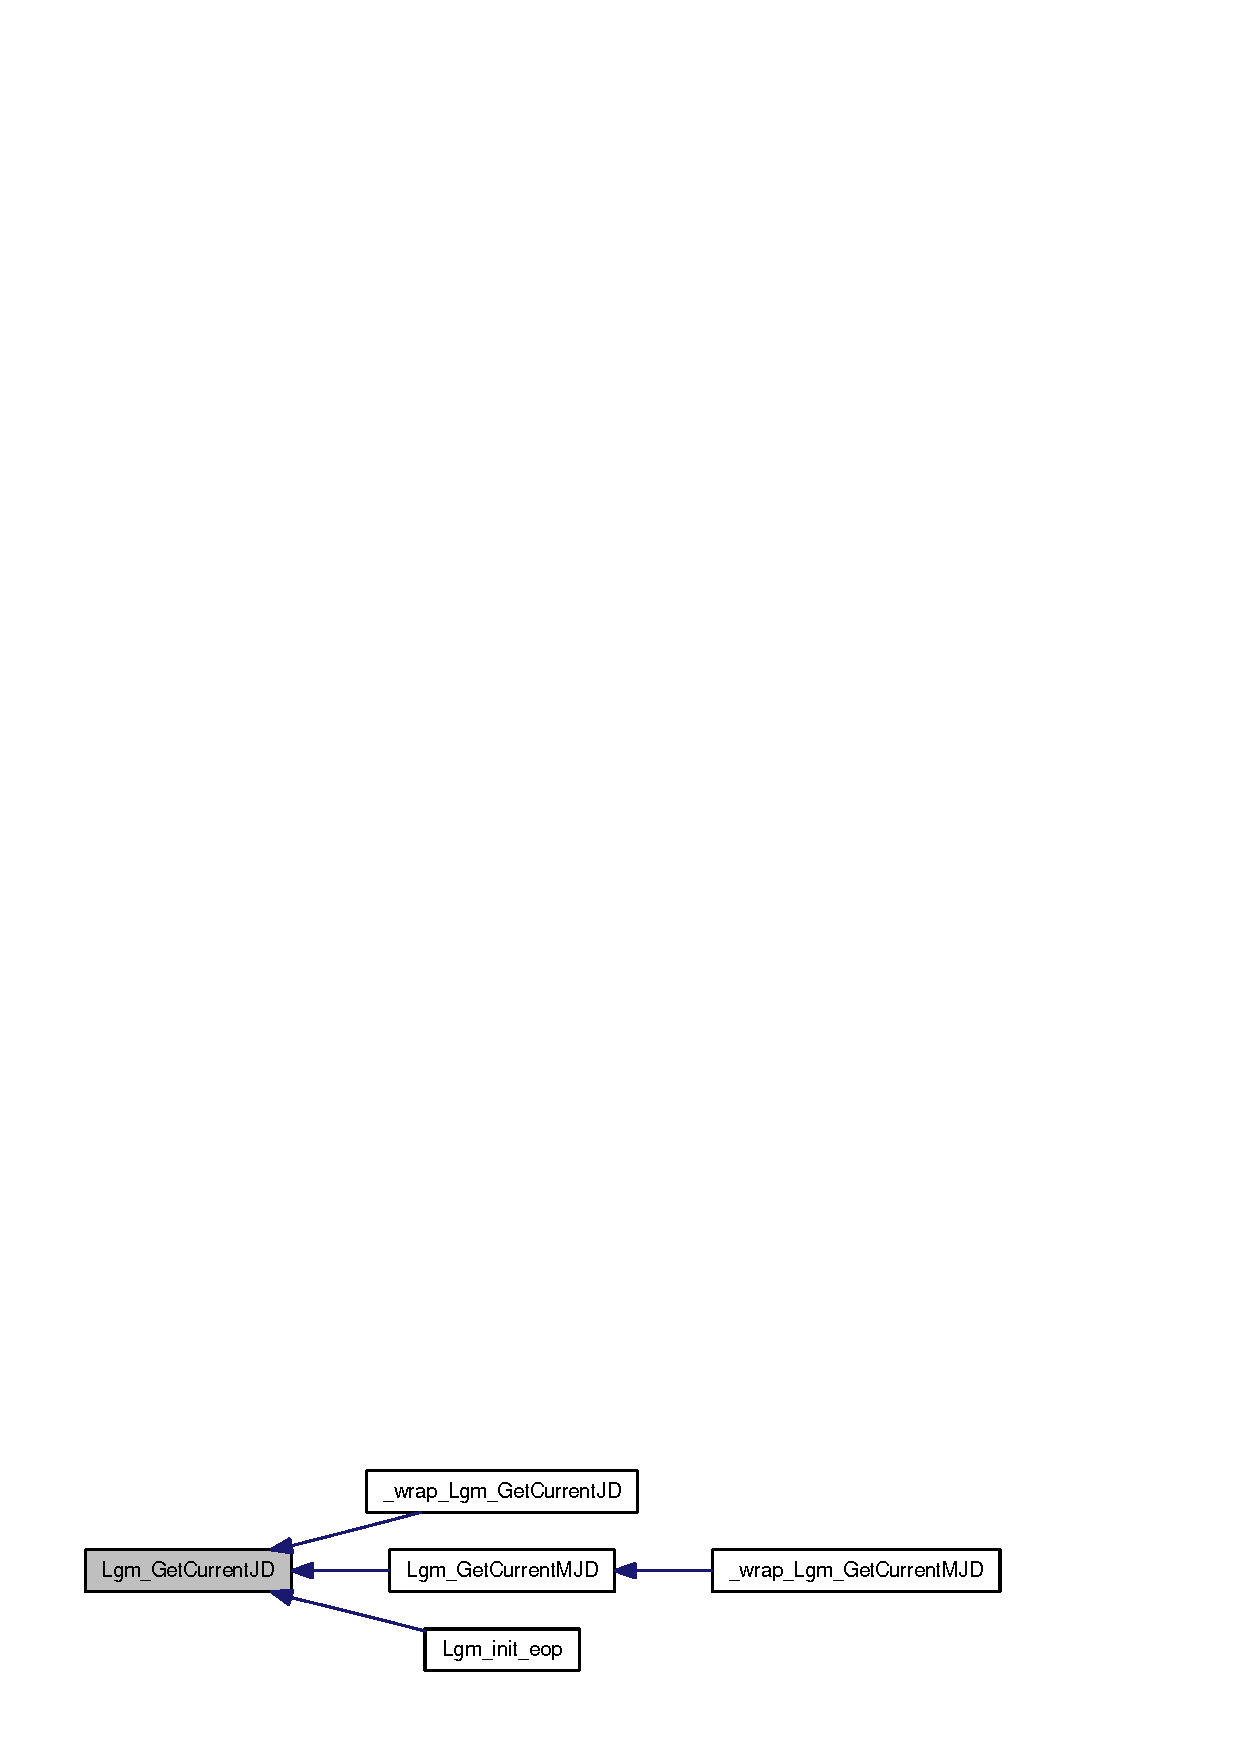
\includegraphics[width=242pt]{_lgm___c_trans_8c_8282c3981409facddb1146c8a38a6473_icgraph}
\end{center}
\end{figure}
\hypertarget{_lgm___c_trans_8c_cb69b434aa7af16c67eadb8679d700fc}{
\index{Lgm\_\-CTrans.c@{Lgm\_\-CTrans.c}!Lgm\_\-GetCurrentMJD@{Lgm\_\-GetCurrentMJD}}
\index{Lgm\_\-GetCurrentMJD@{Lgm\_\-GetCurrentMJD}!Lgm_CTrans.c@{Lgm\_\-CTrans.c}}
\subsubsection[{Lgm\_\-GetCurrentMJD}]{\setlength{\rightskip}{0pt plus 5cm}double Lgm\_\-GetCurrentMJD ({\bf Lgm\_\-CTrans} $\ast$ {\em c})}}
\label{_lgm___c_trans_8c_cb69b434aa7af16c67eadb8679d700fc}




Definition at line 1715 of file Lgm\_\-CTrans.c.

Here is the call graph for this function:\nopagebreak
\begin{figure}[H]
\begin{center}
\leavevmode
\includegraphics[width=266pt]{_lgm___c_trans_8c_cb69b434aa7af16c67eadb8679d700fc_cgraph}
\end{center}
\end{figure}


Here is the caller graph for this function:\nopagebreak
\begin{figure}[H]
\begin{center}
\leavevmode
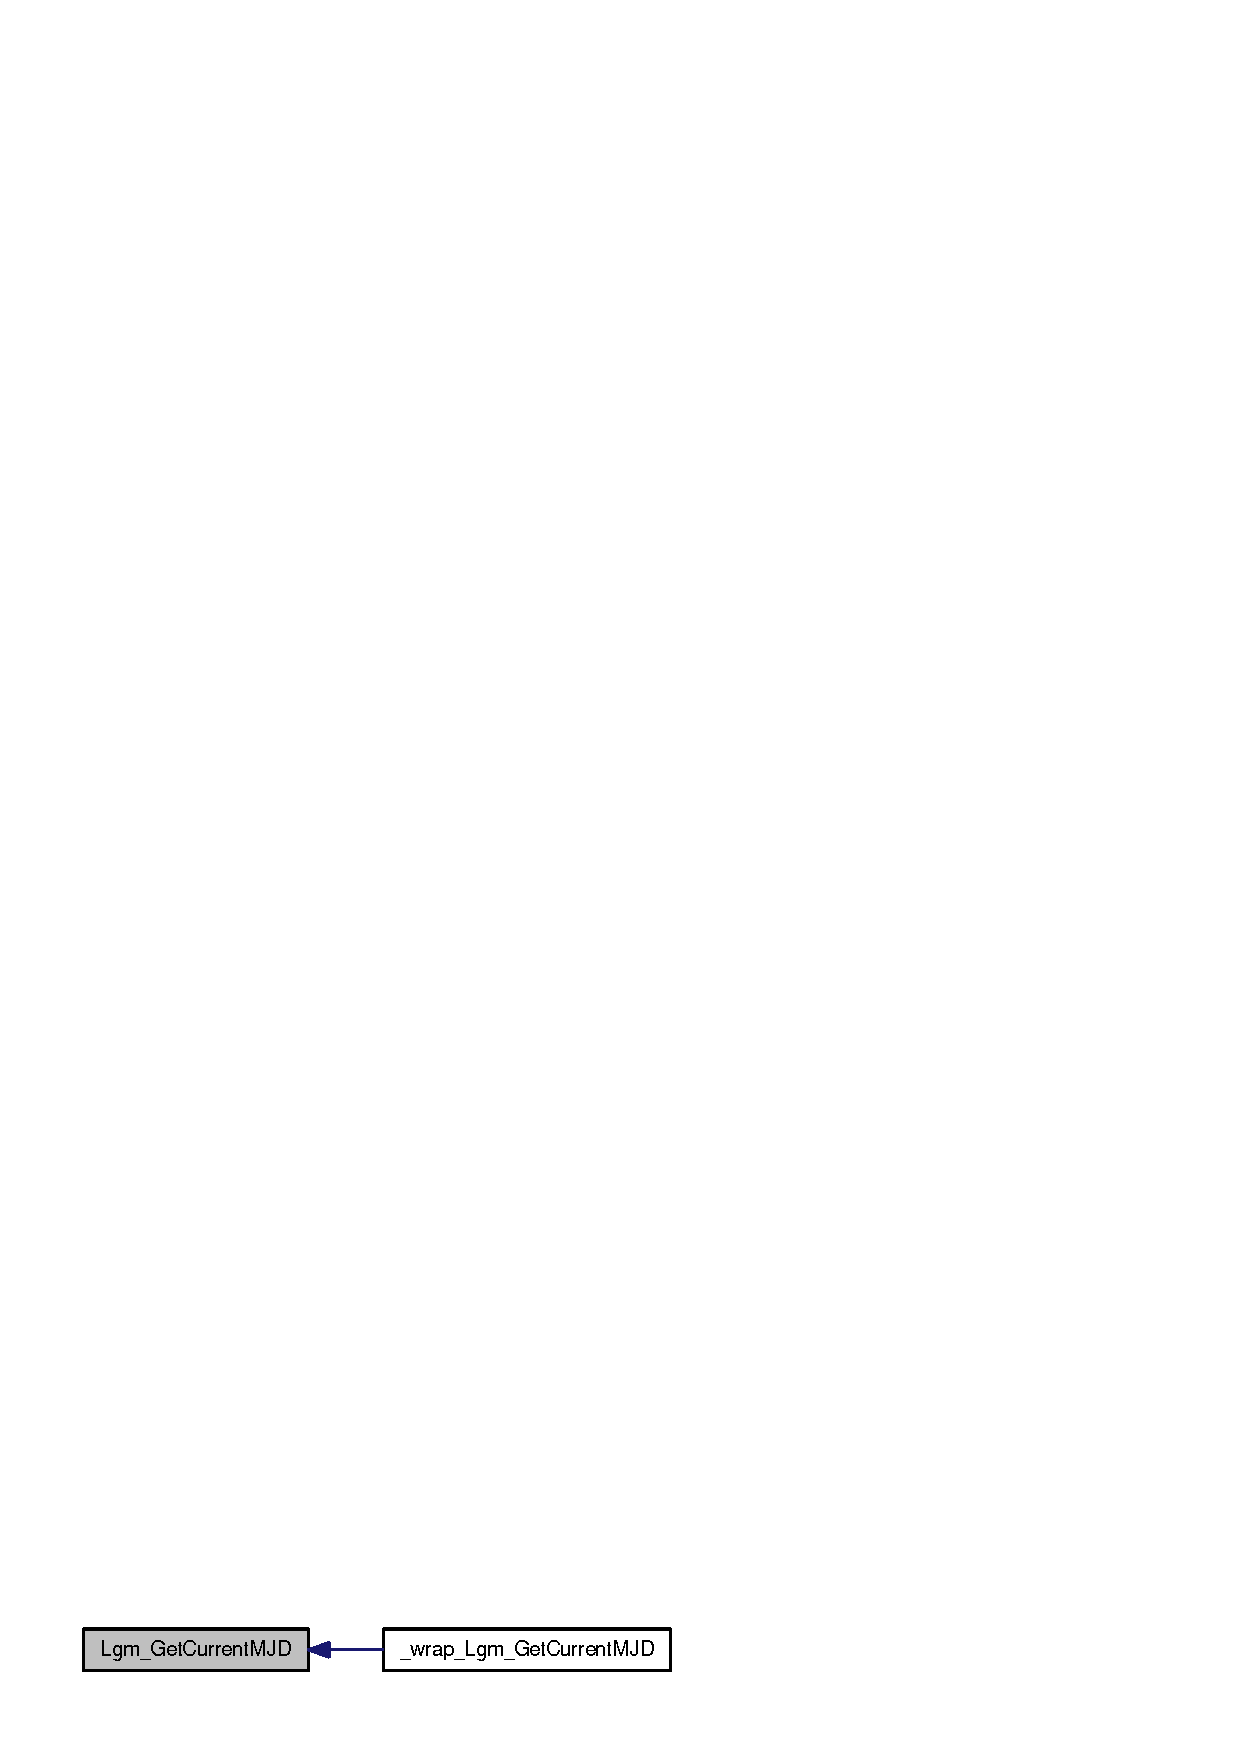
\includegraphics[width=163pt]{_lgm___c_trans_8c_cb69b434aa7af16c67eadb8679d700fc_icgraph}
\end{center}
\end{figure}
\hypertarget{_lgm___c_trans_8c_020fa6e5734e315d2fc9d982263a0f32}{
\index{Lgm\_\-CTrans.c@{Lgm\_\-CTrans.c}!Lgm\_\-Print\_\-HMS@{Lgm\_\-Print\_\-HMS}}
\index{Lgm\_\-Print\_\-HMS@{Lgm\_\-Print\_\-HMS}!Lgm_CTrans.c@{Lgm\_\-CTrans.c}}
\subsubsection[{Lgm\_\-Print\_\-HMS}]{\setlength{\rightskip}{0pt plus 5cm}void Lgm\_\-Print\_\-HMS (double {\em d})}}
\label{_lgm___c_trans_8c_020fa6e5734e315d2fc9d982263a0f32}




Definition at line 1721 of file Lgm\_\-CTrans.c.

Here is the call graph for this function:\nopagebreak
\begin{figure}[H]
\begin{center}
\leavevmode
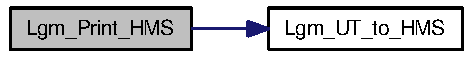
\includegraphics[width=131pt]{_lgm___c_trans_8c_020fa6e5734e315d2fc9d982263a0f32_cgraph}
\end{center}
\end{figure}


Here is the caller graph for this function:\nopagebreak
\begin{figure}[H]
\begin{center}
\leavevmode
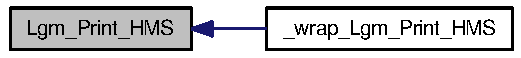
\includegraphics[width=143pt]{_lgm___c_trans_8c_020fa6e5734e315d2fc9d982263a0f32_icgraph}
\end{center}
\end{figure}
\hypertarget{_lgm___c_trans_8c_8c54f2ea495708f306d69eb5cbd5407f}{
\index{Lgm\_\-CTrans.c@{Lgm\_\-CTrans.c}!Lgm\_\-Print\_\-HMSdp@{Lgm\_\-Print\_\-HMSdp}}
\index{Lgm\_\-Print\_\-HMSdp@{Lgm\_\-Print\_\-HMSdp}!Lgm_CTrans.c@{Lgm\_\-CTrans.c}}
\subsubsection[{Lgm\_\-Print\_\-HMSdp}]{\setlength{\rightskip}{0pt plus 5cm}void Lgm\_\-Print\_\-HMSdp (double {\em d}, \/  int {\em UnicodeHMS}, \/  int {\em p})}}
\label{_lgm___c_trans_8c_8c54f2ea495708f306d69eb5cbd5407f}




Definition at line 1737 of file Lgm\_\-CTrans.c.

Here is the call graph for this function:\nopagebreak
\begin{figure}[H]
\begin{center}
\leavevmode
\includegraphics[width=139pt]{_lgm___c_trans_8c_8c54f2ea495708f306d69eb5cbd5407f_cgraph}
\end{center}
\end{figure}


Here is the caller graph for this function:\nopagebreak
\begin{figure}[H]
\begin{center}
\leavevmode
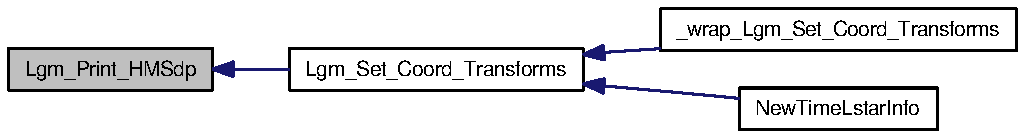
\includegraphics[width=264pt]{_lgm___c_trans_8c_8c54f2ea495708f306d69eb5cbd5407f_icgraph}
\end{center}
\end{figure}
\hypertarget{_lgm___c_trans_8c_09be79dfd1f30dc8313931e19bfb2b68}{
\index{Lgm\_\-CTrans.c@{Lgm\_\-CTrans.c}!Lgm\_\-Print\_\-HMSd@{Lgm\_\-Print\_\-HMSd}}
\index{Lgm\_\-Print\_\-HMSd@{Lgm\_\-Print\_\-HMSd}!Lgm_CTrans.c@{Lgm\_\-CTrans.c}}
\subsubsection[{Lgm\_\-Print\_\-HMSd}]{\setlength{\rightskip}{0pt plus 5cm}void Lgm\_\-Print\_\-HMSd (double {\em d})}}
\label{_lgm___c_trans_8c_09be79dfd1f30dc8313931e19bfb2b68}




Definition at line 1786 of file Lgm\_\-CTrans.c.

Here is the call graph for this function:\nopagebreak
\begin{figure}[H]
\begin{center}
\leavevmode
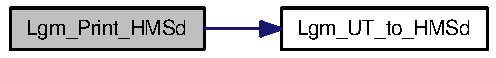
\includegraphics[width=137pt]{_lgm___c_trans_8c_09be79dfd1f30dc8313931e19bfb2b68_cgraph}
\end{center}
\end{figure}


Here is the caller graph for this function:\nopagebreak
\begin{figure}[H]
\begin{center}
\leavevmode
\includegraphics[width=262pt]{_lgm___c_trans_8c_09be79dfd1f30dc8313931e19bfb2b68_icgraph}
\end{center}
\end{figure}
\hypertarget{_lgm___c_trans_8c_c0752451ba731db6f7ad5ff7aa7388cb}{
\index{Lgm\_\-CTrans.c@{Lgm\_\-CTrans.c}!Lgm\_\-Print\_\-DMS@{Lgm\_\-Print\_\-DMS}}
\index{Lgm\_\-Print\_\-DMS@{Lgm\_\-Print\_\-DMS}!Lgm_CTrans.c@{Lgm\_\-CTrans.c}}
\subsubsection[{Lgm\_\-Print\_\-DMS}]{\setlength{\rightskip}{0pt plus 5cm}void Lgm\_\-Print\_\-DMS (double {\em d})}}
\label{_lgm___c_trans_8c_c0752451ba731db6f7ad5ff7aa7388cb}




Definition at line 1802 of file Lgm\_\-CTrans.c.

Here is the call graph for this function:\nopagebreak
\begin{figure}[H]
\begin{center}
\leavevmode
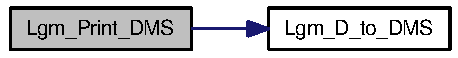
\includegraphics[width=128pt]{_lgm___c_trans_8c_c0752451ba731db6f7ad5ff7aa7388cb_cgraph}
\end{center}
\end{figure}


Here is the caller graph for this function:\nopagebreak
\begin{figure}[H]
\begin{center}
\leavevmode
\includegraphics[width=143pt]{_lgm___c_trans_8c_c0752451ba731db6f7ad5ff7aa7388cb_icgraph}
\end{center}
\end{figure}
\hypertarget{_lgm___c_trans_8c_0f6fd0c4c8d56743de4c9e24039eb1df}{
\index{Lgm\_\-CTrans.c@{Lgm\_\-CTrans.c}!Lgm\_\-Print\_\-DMSd@{Lgm\_\-Print\_\-DMSd}}
\index{Lgm\_\-Print\_\-DMSd@{Lgm\_\-Print\_\-DMSd}!Lgm_CTrans.c@{Lgm\_\-CTrans.c}}
\subsubsection[{Lgm\_\-Print\_\-DMSd}]{\setlength{\rightskip}{0pt plus 5cm}void Lgm\_\-Print\_\-DMSd (double {\em d})}}
\label{_lgm___c_trans_8c_0f6fd0c4c8d56743de4c9e24039eb1df}




Definition at line 1810 of file Lgm\_\-CTrans.c.

Here is the call graph for this function:\nopagebreak
\begin{figure}[H]
\begin{center}
\leavevmode
\includegraphics[width=134pt]{_lgm___c_trans_8c_0f6fd0c4c8d56743de4c9e24039eb1df_cgraph}
\end{center}
\end{figure}


Here is the caller graph for this function:\nopagebreak
\begin{figure}[H]
\begin{center}
\leavevmode
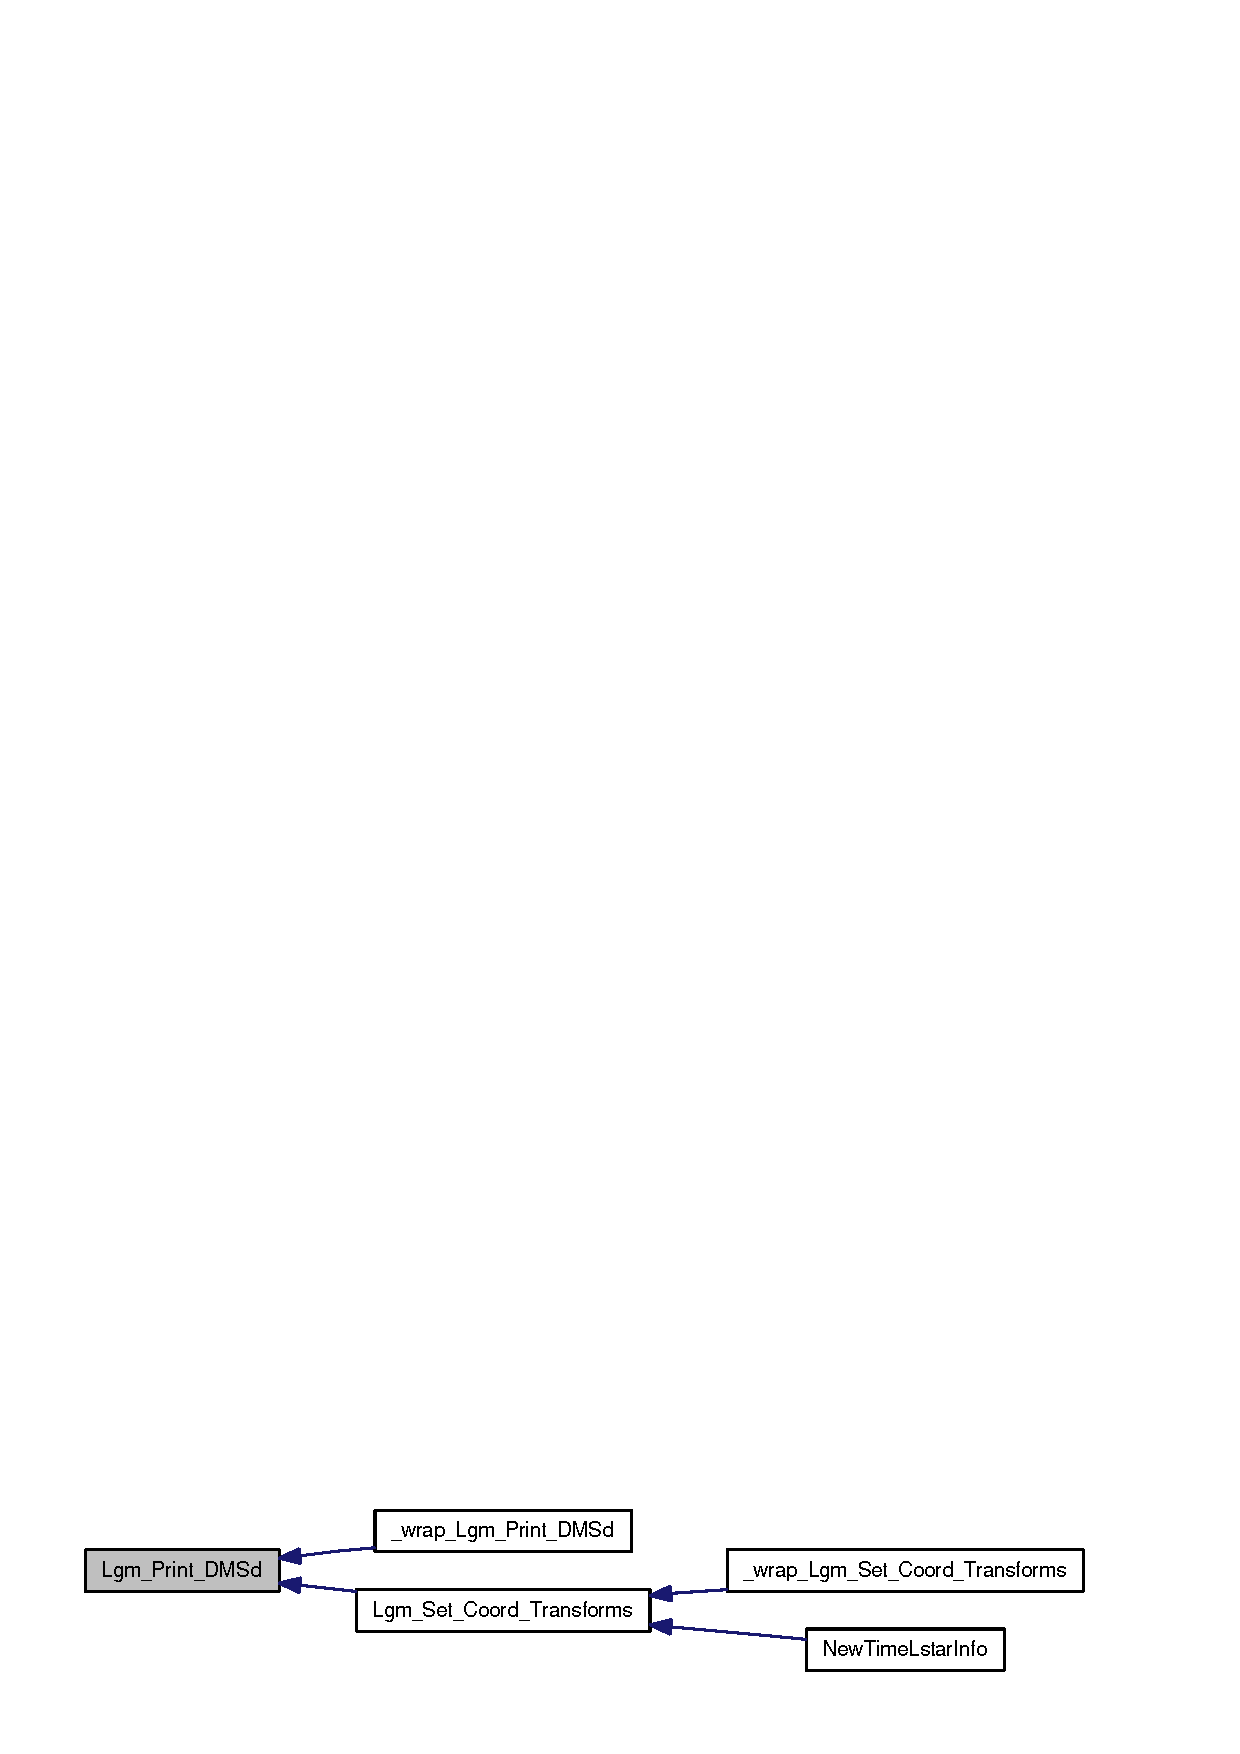
\includegraphics[width=262pt]{_lgm___c_trans_8c_0f6fd0c4c8d56743de4c9e24039eb1df_icgraph}
\end{center}
\end{figure}
\hypertarget{_lgm___c_trans_8c_022c69d1faa38210aba90d732e3b4327}{
\index{Lgm\_\-CTrans.c@{Lgm\_\-CTrans.c}!Lgm\_\-CDMAG\_\-to\_\-R\_\-MLAT\_\-MLON\_\-MLT@{Lgm\_\-CDMAG\_\-to\_\-R\_\-MLAT\_\-MLON\_\-MLT}}
\index{Lgm\_\-CDMAG\_\-to\_\-R\_\-MLAT\_\-MLON\_\-MLT@{Lgm\_\-CDMAG\_\-to\_\-R\_\-MLAT\_\-MLON\_\-MLT}!Lgm_CTrans.c@{Lgm\_\-CTrans.c}}
\subsubsection[{Lgm\_\-CDMAG\_\-to\_\-R\_\-MLAT\_\-MLON\_\-MLT}]{\setlength{\rightskip}{0pt plus 5cm}void Lgm\_\-CDMAG\_\-to\_\-R\_\-MLAT\_\-MLON\_\-MLT ({\bf Lgm\_\-Vector} $\ast$ {\em u}, \/  double $\ast$ {\em R}, \/  double $\ast$ {\em MLAT}, \/  double $\ast$ {\em MLON}, \/  double $\ast$ {\em MLT}, \/  {\bf Lgm\_\-CTrans} $\ast$ {\em c})}}
\label{_lgm___c_trans_8c_022c69d1faa38210aba90d732e3b4327}




Definition at line 1827 of file Lgm\_\-CTrans.c.

Here is the call graph for this function:\nopagebreak
\begin{figure}[H]
\begin{center}
\leavevmode
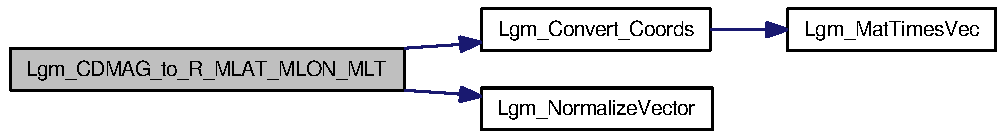
\includegraphics[width=259pt]{_lgm___c_trans_8c_022c69d1faa38210aba90d732e3b4327_cgraph}
\end{center}
\end{figure}


Here is the caller graph for this function:\nopagebreak
\begin{figure}[H]
\begin{center}
\leavevmode
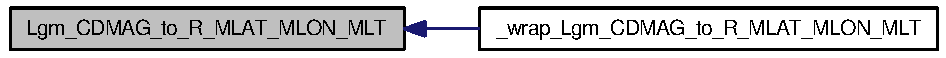
\includegraphics[width=245pt]{_lgm___c_trans_8c_022c69d1faa38210aba90d732e3b4327_icgraph}
\end{center}
\end{figure}
\hypertarget{_lgm___c_trans_8c_b266f1ac29eac32ae2bc43c92514a8c1}{
\index{Lgm\_\-CTrans.c@{Lgm\_\-CTrans.c}!Lgm\_\-R\_\-MLAT\_\-MLT\_\-to\_\-CDMAG@{Lgm\_\-R\_\-MLAT\_\-MLT\_\-to\_\-CDMAG}}
\index{Lgm\_\-R\_\-MLAT\_\-MLT\_\-to\_\-CDMAG@{Lgm\_\-R\_\-MLAT\_\-MLT\_\-to\_\-CDMAG}!Lgm_CTrans.c@{Lgm\_\-CTrans.c}}
\subsubsection[{Lgm\_\-R\_\-MLAT\_\-MLT\_\-to\_\-CDMAG}]{\setlength{\rightskip}{0pt plus 5cm}void Lgm\_\-R\_\-MLAT\_\-MLT\_\-to\_\-CDMAG (double {\em R}, \/  double {\em MLAT}, \/  double {\em MLT}, \/  {\bf Lgm\_\-Vector} $\ast$ {\em u}, \/  {\bf Lgm\_\-CTrans} $\ast$ {\em c})}}
\label{_lgm___c_trans_8c_b266f1ac29eac32ae2bc43c92514a8c1}




Definition at line 1861 of file Lgm\_\-CTrans.c.

Here is the call graph for this function:\nopagebreak
\begin{figure}[H]
\begin{center}
\leavevmode
\includegraphics[width=242pt]{_lgm___c_trans_8c_b266f1ac29eac32ae2bc43c92514a8c1_cgraph}
\end{center}
\end{figure}


Here is the caller graph for this function:\nopagebreak
\begin{figure}[H]
\begin{center}
\leavevmode
\includegraphics[width=213pt]{_lgm___c_trans_8c_b266f1ac29eac32ae2bc43c92514a8c1_icgraph}
\end{center}
\end{figure}
\hypertarget{_lgm___c_trans_8c_ffd68c7f63f3835e4b941894d7970036}{
\index{Lgm\_\-CTrans.c@{Lgm\_\-CTrans.c}!Lgm\_\-EDMAG\_\-to\_\-R\_\-MLAT\_\-MLON\_\-MLT@{Lgm\_\-EDMAG\_\-to\_\-R\_\-MLAT\_\-MLON\_\-MLT}}
\index{Lgm\_\-EDMAG\_\-to\_\-R\_\-MLAT\_\-MLON\_\-MLT@{Lgm\_\-EDMAG\_\-to\_\-R\_\-MLAT\_\-MLON\_\-MLT}!Lgm_CTrans.c@{Lgm\_\-CTrans.c}}
\subsubsection[{Lgm\_\-EDMAG\_\-to\_\-R\_\-MLAT\_\-MLON\_\-MLT}]{\setlength{\rightskip}{0pt plus 5cm}void Lgm\_\-EDMAG\_\-to\_\-R\_\-MLAT\_\-MLON\_\-MLT ({\bf Lgm\_\-Vector} $\ast$ {\em u}, \/  double $\ast$ {\em R}, \/  double $\ast$ {\em MLAT}, \/  double $\ast$ {\em MLON}, \/  double $\ast$ {\em MLT}, \/  {\bf Lgm\_\-CTrans} $\ast$ {\em c})}}
\label{_lgm___c_trans_8c_ffd68c7f63f3835e4b941894d7970036}




Definition at line 1889 of file Lgm\_\-CTrans.c.

Here is the call graph for this function:\nopagebreak
\begin{figure}[H]
\begin{center}
\leavevmode
\includegraphics[width=259pt]{_lgm___c_trans_8c_ffd68c7f63f3835e4b941894d7970036_cgraph}
\end{center}
\end{figure}


Here is the caller graph for this function:\nopagebreak
\begin{figure}[H]
\begin{center}
\leavevmode
\includegraphics[width=245pt]{_lgm___c_trans_8c_ffd68c7f63f3835e4b941894d7970036_icgraph}
\end{center}
\end{figure}
\hypertarget{_lgm___c_trans_8c_990e8076d81fa9fb61683eadba58f948}{
\index{Lgm\_\-CTrans.c@{Lgm\_\-CTrans.c}!Lgm\_\-R\_\-MLAT\_\-MLT\_\-to\_\-EDMAG@{Lgm\_\-R\_\-MLAT\_\-MLT\_\-to\_\-EDMAG}}
\index{Lgm\_\-R\_\-MLAT\_\-MLT\_\-to\_\-EDMAG@{Lgm\_\-R\_\-MLAT\_\-MLT\_\-to\_\-EDMAG}!Lgm_CTrans.c@{Lgm\_\-CTrans.c}}
\subsubsection[{Lgm\_\-R\_\-MLAT\_\-MLT\_\-to\_\-EDMAG}]{\setlength{\rightskip}{0pt plus 5cm}void Lgm\_\-R\_\-MLAT\_\-MLT\_\-to\_\-EDMAG (double {\em R}, \/  double {\em MLAT}, \/  double {\em MLT}, \/  {\bf Lgm\_\-Vector} $\ast$ {\em u}, \/  {\bf Lgm\_\-CTrans} $\ast$ {\em c})}}
\label{_lgm___c_trans_8c_990e8076d81fa9fb61683eadba58f948}




Definition at line 1920 of file Lgm\_\-CTrans.c.

Here is the call graph for this function:\nopagebreak
\begin{figure}[H]
\begin{center}
\leavevmode
\includegraphics[width=242pt]{_lgm___c_trans_8c_990e8076d81fa9fb61683eadba58f948_cgraph}
\end{center}
\end{figure}


Here is the caller graph for this function:\nopagebreak
\begin{figure}[H]
\begin{center}
\leavevmode
\includegraphics[width=213pt]{_lgm___c_trans_8c_990e8076d81fa9fb61683eadba58f948_icgraph}
\end{center}
\end{figure}
\hypertarget{_lgm___c_trans_8c_ac416039271e229bfe94fd9f7b610dc5}{
\index{Lgm\_\-CTrans.c@{Lgm\_\-CTrans.c}!Lgm\_\-GLATLON\_\-TO\_\-CDMLATLONMLT@{Lgm\_\-GLATLON\_\-TO\_\-CDMLATLONMLT}}
\index{Lgm\_\-GLATLON\_\-TO\_\-CDMLATLONMLT@{Lgm\_\-GLATLON\_\-TO\_\-CDMLATLONMLT}!Lgm_CTrans.c@{Lgm\_\-CTrans.c}}
\subsubsection[{Lgm\_\-GLATLON\_\-TO\_\-CDMLATLONMLT}]{\setlength{\rightskip}{0pt plus 5cm}void Lgm\_\-GLATLON\_\-TO\_\-CDMLATLONMLT (double {\em GLAT}, \/  double {\em GLON}, \/  double $\ast$ {\em MLAT}, \/  double $\ast$ {\em MLON}, \/  double $\ast$ {\em MLT}, \/  {\bf Lgm\_\-CTrans} $\ast$ {\em c})}}
\label{_lgm___c_trans_8c_ac416039271e229bfe94fd9f7b610dc5}




Definition at line 1948 of file Lgm\_\-CTrans.c.

Here is the call graph for this function:\nopagebreak
\begin{figure}[H]
\begin{center}
\leavevmode
\includegraphics[width=256pt]{_lgm___c_trans_8c_ac416039271e229bfe94fd9f7b610dc5_cgraph}
\end{center}
\end{figure}


Here is the caller graph for this function:\nopagebreak
\begin{figure}[H]
\begin{center}
\leavevmode
\includegraphics[width=241pt]{_lgm___c_trans_8c_ac416039271e229bfe94fd9f7b610dc5_icgraph}
\end{center}
\end{figure}
\hypertarget{_lgm___c_trans_8c_cd9faa6a7bfbe63a8b4ece64e9940d3d}{
\index{Lgm\_\-CTrans.c@{Lgm\_\-CTrans.c}!Lgm\_\-GLATLON\_\-TO\_\-EDMLATLONMLT@{Lgm\_\-GLATLON\_\-TO\_\-EDMLATLONMLT}}
\index{Lgm\_\-GLATLON\_\-TO\_\-EDMLATLONMLT@{Lgm\_\-GLATLON\_\-TO\_\-EDMLATLONMLT}!Lgm_CTrans.c@{Lgm\_\-CTrans.c}}
\subsubsection[{Lgm\_\-GLATLON\_\-TO\_\-EDMLATLONMLT}]{\setlength{\rightskip}{0pt plus 5cm}void Lgm\_\-GLATLON\_\-TO\_\-EDMLATLONMLT (double {\em GLAT}, \/  double {\em GLON}, \/  double $\ast$ {\em MLAT}, \/  double $\ast$ {\em MLON}, \/  double $\ast$ {\em MLT}, \/  {\bf Lgm\_\-CTrans} $\ast$ {\em c})}}
\label{_lgm___c_trans_8c_cd9faa6a7bfbe63a8b4ece64e9940d3d}




Definition at line 1981 of file Lgm\_\-CTrans.c.

Here is the call graph for this function:\nopagebreak
\begin{figure}[H]
\begin{center}
\leavevmode
\includegraphics[width=256pt]{_lgm___c_trans_8c_cd9faa6a7bfbe63a8b4ece64e9940d3d_cgraph}
\end{center}
\end{figure}


Here is the caller graph for this function:\nopagebreak
\begin{figure}[H]
\begin{center}
\leavevmode
\includegraphics[width=241pt]{_lgm___c_trans_8c_cd9faa6a7bfbe63a8b4ece64e9940d3d_icgraph}
\end{center}
\end{figure}
\hypertarget{_lgm___c_trans_8c_6451734bb5156adb8f3dcff4f699f6c6}{
\index{Lgm\_\-CTrans.c@{Lgm\_\-CTrans.c}!ParseTimeStr@{ParseTimeStr}}
\index{ParseTimeStr@{ParseTimeStr}!Lgm_CTrans.c@{Lgm\_\-CTrans.c}}
\subsubsection[{ParseTimeStr}]{\setlength{\rightskip}{0pt plus 5cm}void ParseTimeStr (char $\ast$ {\em Str}, \/  int $\ast$ {\em Year}, \/  int $\ast$ {\em Month}, \/  int $\ast$ {\em Day}, \/  int $\ast$ {\em hh}, \/  int $\ast$ {\em mm}, \/  double $\ast$ {\em ss}, \/  long int $\ast$ {\em Date}, \/  double $\ast$ {\em H})}}
\label{_lgm___c_trans_8c_6451734bb5156adb8f3dcff4f699f6c6}




Definition at line 2012 of file Lgm\_\-CTrans.c.

Here is the call graph for this function:\nopagebreak
\begin{figure}[H]
\begin{center}
\leavevmode
\includegraphics[width=185pt]{_lgm___c_trans_8c_6451734bb5156adb8f3dcff4f699f6c6_cgraph}
\end{center}
\end{figure}
\hypertarget{_lgm___c_trans_8c_d1aa3133c642d6449d82195218a982d7}{
\index{Lgm\_\-CTrans.c@{Lgm\_\-CTrans.c}!MonthStrToNum@{MonthStrToNum}}
\index{MonthStrToNum@{MonthStrToNum}!Lgm_CTrans.c@{Lgm\_\-CTrans.c}}
\subsubsection[{MonthStrToNum}]{\setlength{\rightskip}{0pt plus 5cm}int MonthStrToNum (char $\ast$ {\em str})}}
\label{_lgm___c_trans_8c_d1aa3133c642d6449d82195218a982d7}




Definition at line 2023 of file Lgm\_\-CTrans.c.

Here is the call graph for this function:\nopagebreak
\begin{figure}[H]
\begin{center}
\leavevmode
\includegraphics[width=129pt]{_lgm___c_trans_8c_d1aa3133c642d6449d82195218a982d7_cgraph}
\end{center}
\end{figure}


Here is the caller graph for this function:\nopagebreak
\begin{figure}[H]
\begin{center}
\leavevmode
\includegraphics[width=122pt]{_lgm___c_trans_8c_d1aa3133c642d6449d82195218a982d7_icgraph}
\end{center}
\end{figure}
\hypertarget{_lgm___c_trans_8c_a235edbf150af5c6ad528c6a6f549776}{
\index{Lgm\_\-CTrans.c@{Lgm\_\-CTrans.c}!Lgm\_\-StrToLower@{Lgm\_\-StrToLower}}
\index{Lgm\_\-StrToLower@{Lgm\_\-StrToLower}!Lgm_CTrans.c@{Lgm\_\-CTrans.c}}
\subsubsection[{Lgm\_\-StrToLower}]{\setlength{\rightskip}{0pt plus 5cm}char$\ast$ Lgm\_\-StrToLower (char $\ast$ {\em str}, \/  int {\em nmax})}}
\label{_lgm___c_trans_8c_a235edbf150af5c6ad528c6a6f549776}




Definition at line 2041 of file Lgm\_\-CTrans.c.

Here is the caller graph for this function:\nopagebreak
\begin{figure}[H]
\begin{center}
\leavevmode
\includegraphics[width=185pt]{_lgm___c_trans_8c_a235edbf150af5c6ad528c6a6f549776_icgraph}
\end{center}
\end{figure}
\hypertarget{_lgm___c_trans_8c_aab1a57905dff35bc1efeef8c3f6a576}{
\index{Lgm\_\-CTrans.c@{Lgm\_\-CTrans.c}!Lgm\_\-StrToUpper@{Lgm\_\-StrToUpper}}
\index{Lgm\_\-StrToUpper@{Lgm\_\-StrToUpper}!Lgm_CTrans.c@{Lgm\_\-CTrans.c}}
\subsubsection[{Lgm\_\-StrToUpper}]{\setlength{\rightskip}{0pt plus 5cm}char$\ast$ Lgm\_\-StrToUpper (char $\ast$ {\em str}, \/  int {\em nmax})}}
\label{_lgm___c_trans_8c_aab1a57905dff35bc1efeef8c3f6a576}




Definition at line 2052 of file Lgm\_\-CTrans.c.